% Activate the following line by filling in the right side. If for example the name of the root file is Main.tex, write
% "...root = Main.tex" if the chapter file is in the same directory, and "...root = ../Main.tex" if the chapter is in a subdirectory.
 
%!TEX root =  ../Thesis.tex

\chapter[Signal Kinematics]{Signal Kinematics}

 
\section{Signal Jet Kinematics}

Once the trigger and cuts have been applied to the data, the events that remain can be signal, background, or a mixture of the two.  
It then falls to understanding the kinematics of the signal and background to look for features that can
provide enough discrimination to detect the presence of the signal.  In this case, that means reconstructing
the invariant mass of the leading 2 jets in the event, which will create a smoothly falling power
law distribution in QCD background but a resonance structure in signal.  The kinematics of the signal
distribution then come into play in a few major ways
\begin{itemize}
    \item Signal Jet \pt Distributions:  By examining the \pt distributions of the Higgs daughters, and the associated $b$-jet(s), we can get a better understanding of what might be optimal jet \pt cuts for future iterationsof this analysis 
    \item Signal Jet Combinatorics: A perfectly good signal event can be inadvertently turned into a type of background if the associated $b$-jet is chosen when reconstructing the Higgs; unfortunately these combinatorial mistakes can arise easily when there are 3 $b$-jets but only two jets being used for reconstruction
    \item Mass Resolution: The Higgs resonance width is $m_A$/tan$\beta$ dependent, with inherent widths
up to a few tens of GeV; however, if energy is lost to FSR, the resonance can be much wider and this makes
the signal much more difficult to distinguish from the background
\end{itemize}


\section{Signal Jet \pt Distributions}

An important place to start is with the \pt distributions of the jets after the trigger
and cuts have been applied.  Using truth-matching in the Monte Carlo, we can identify
which jets are daughters of the Higgs and which are associated $b$-jet(s).  Since
the Higgs is a heavy particle, its decay jets tend to have higher \pt than the associated
$b$-jet(s), which can be seen in Figure~\ref{fig:pt_higgs_and_associated_jets}. 
However, in this plot, there has been $b$-tagging applied so an important potential
component is missing: how does the event topology change when we also include 
non-$b$-jets, which can potentially be high \pt as well.   

%----------------------------------------------
\begin{figure}[H]
    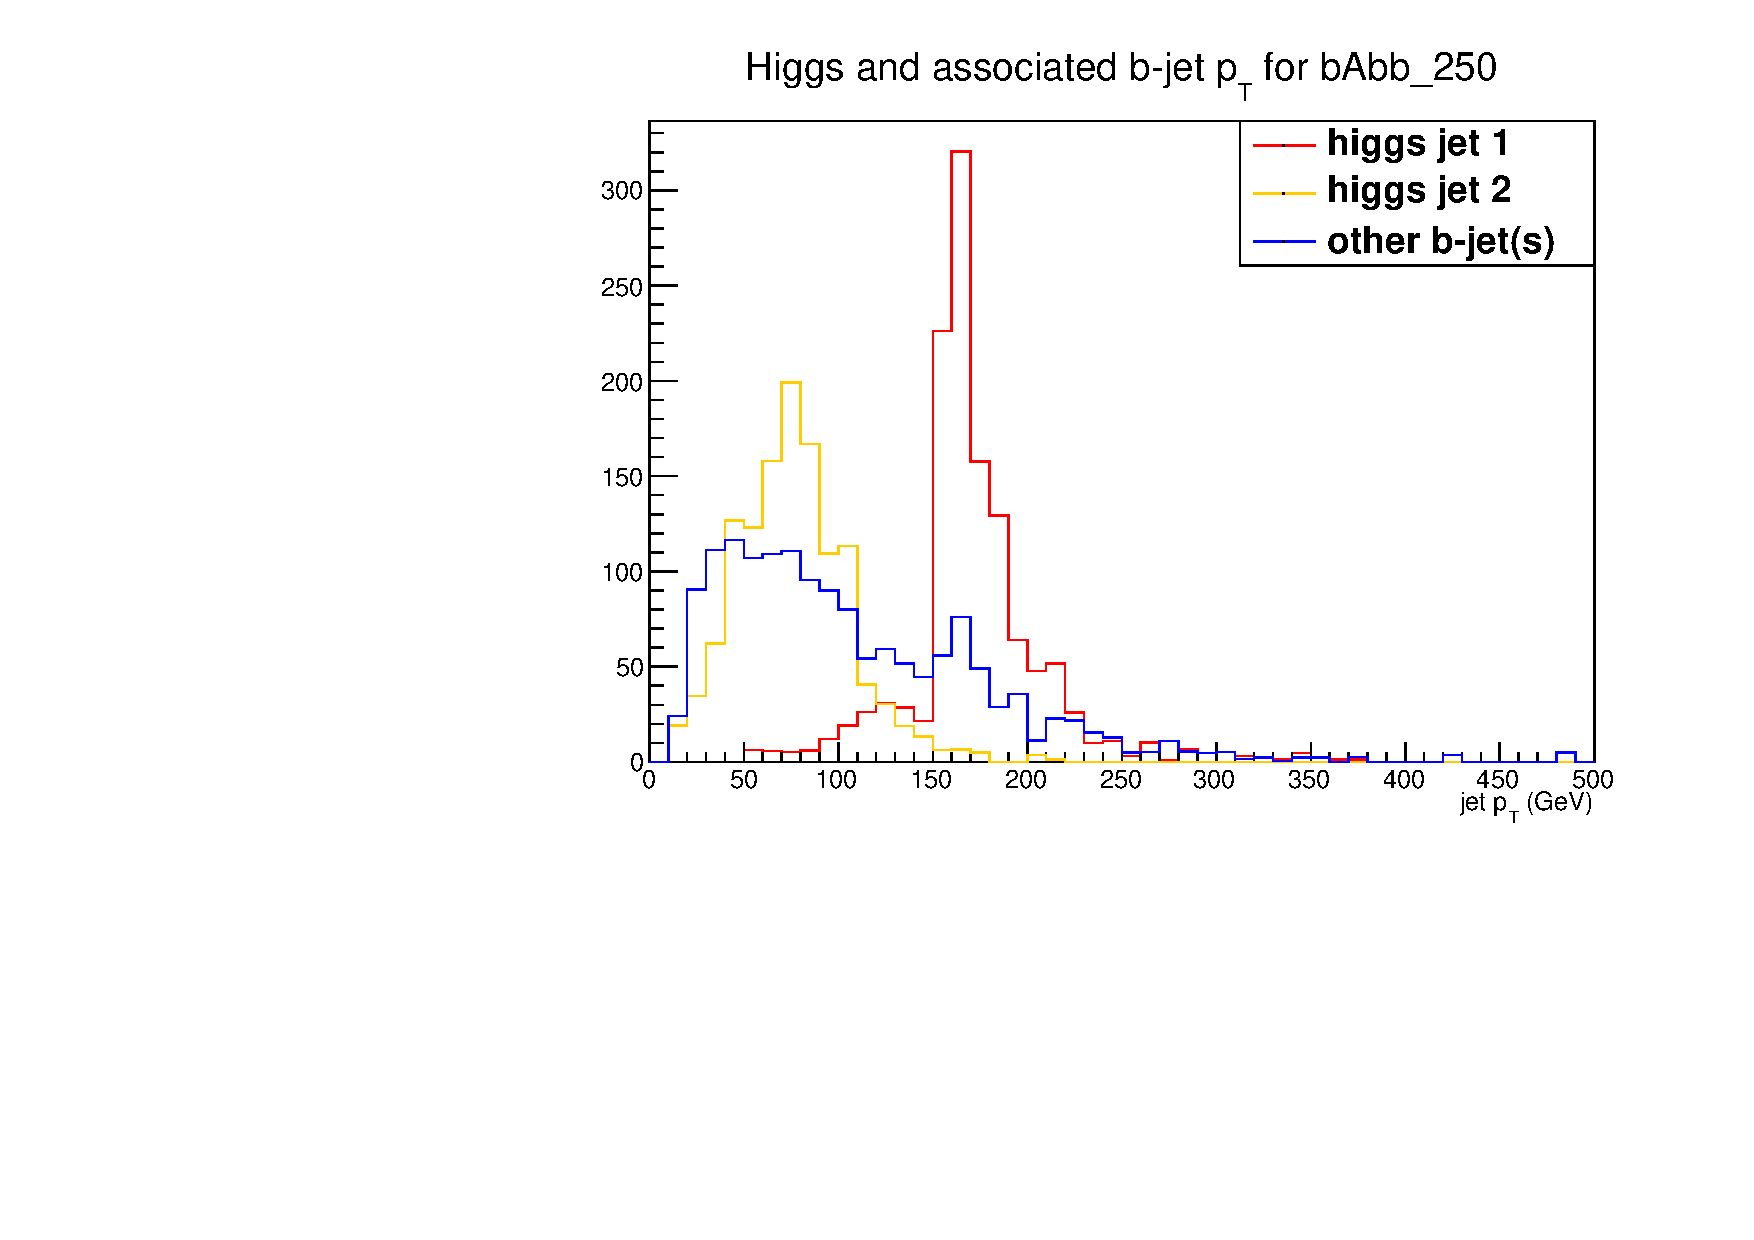
\includegraphics[width=0.3\textwidth]{SignalKin/jet_pt_compare_bAbb_250.pdf}
    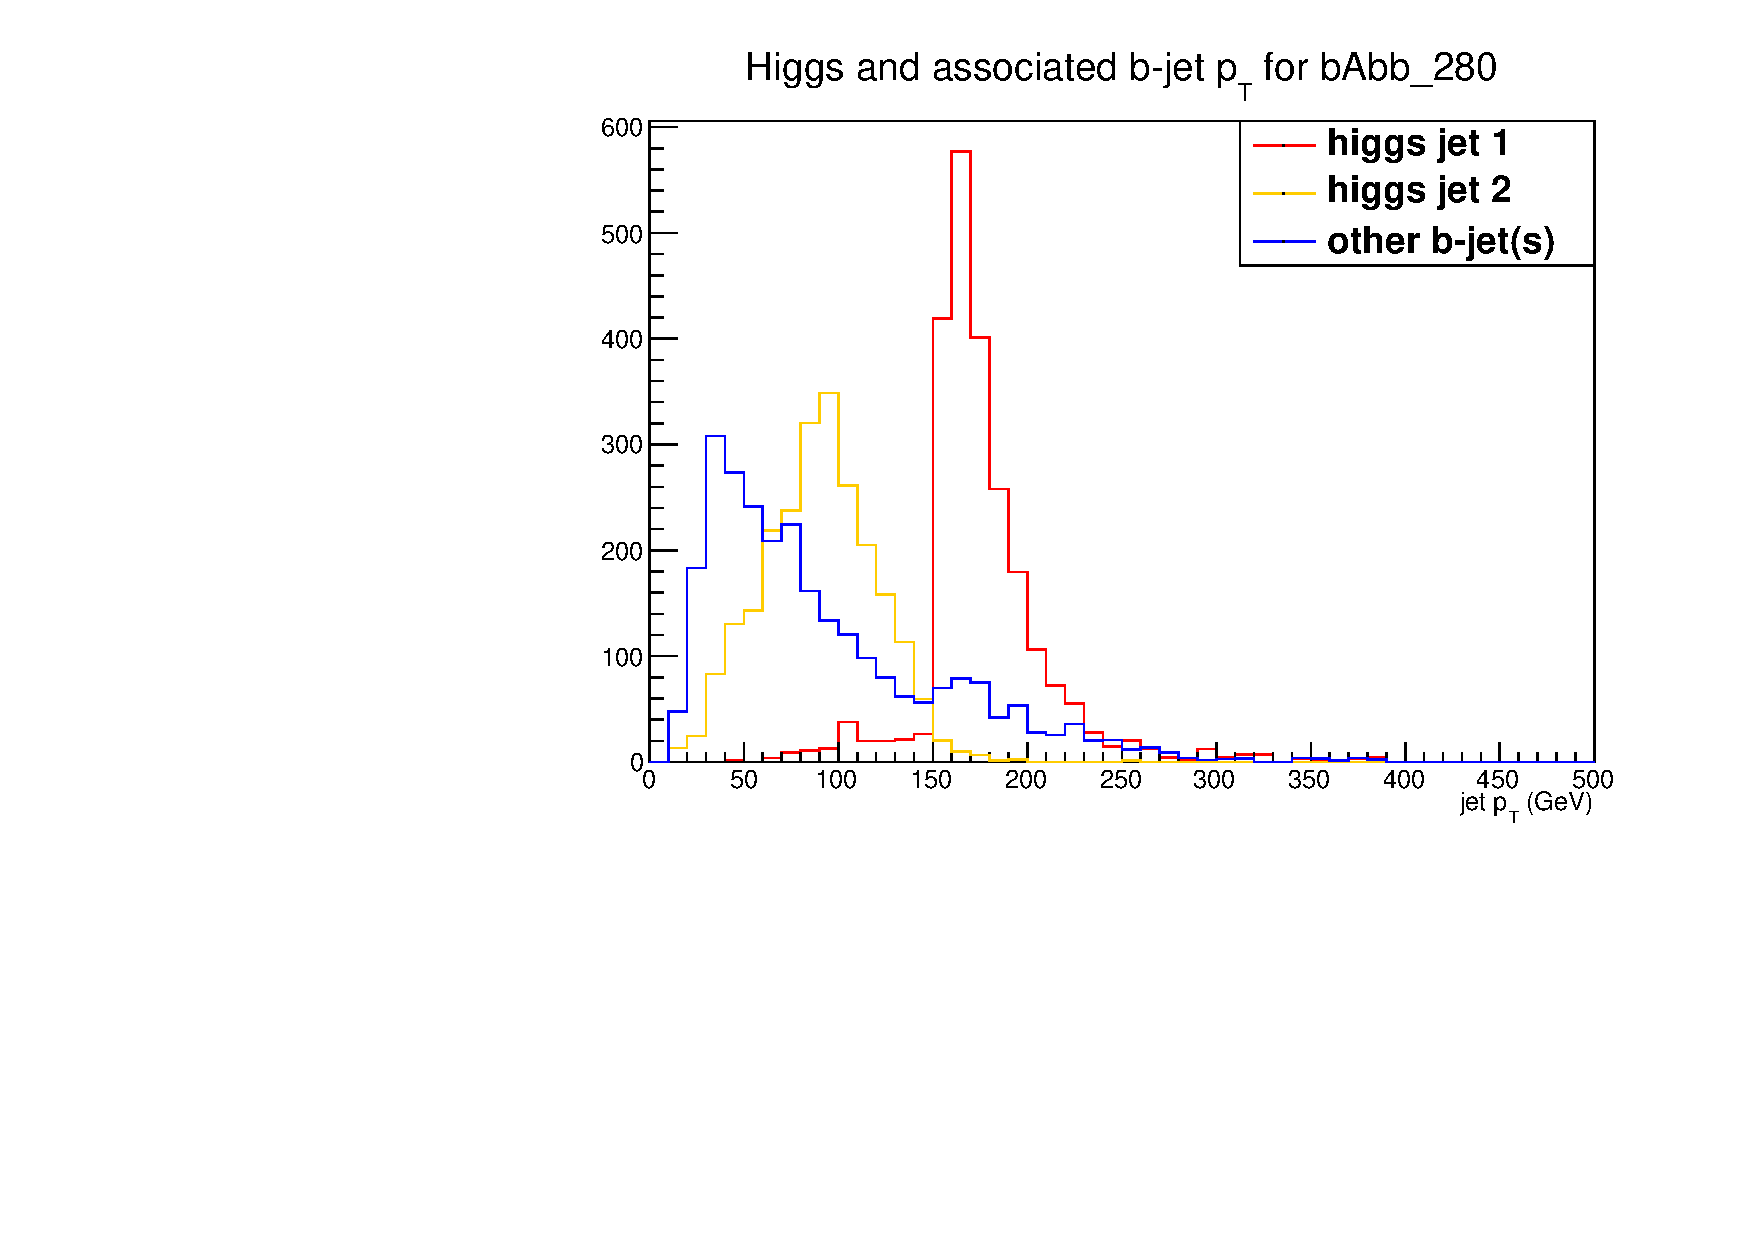
\includegraphics[width=0.3\textwidth]{SignalKin/jet_pt_compare_bAbb_280.pdf}
    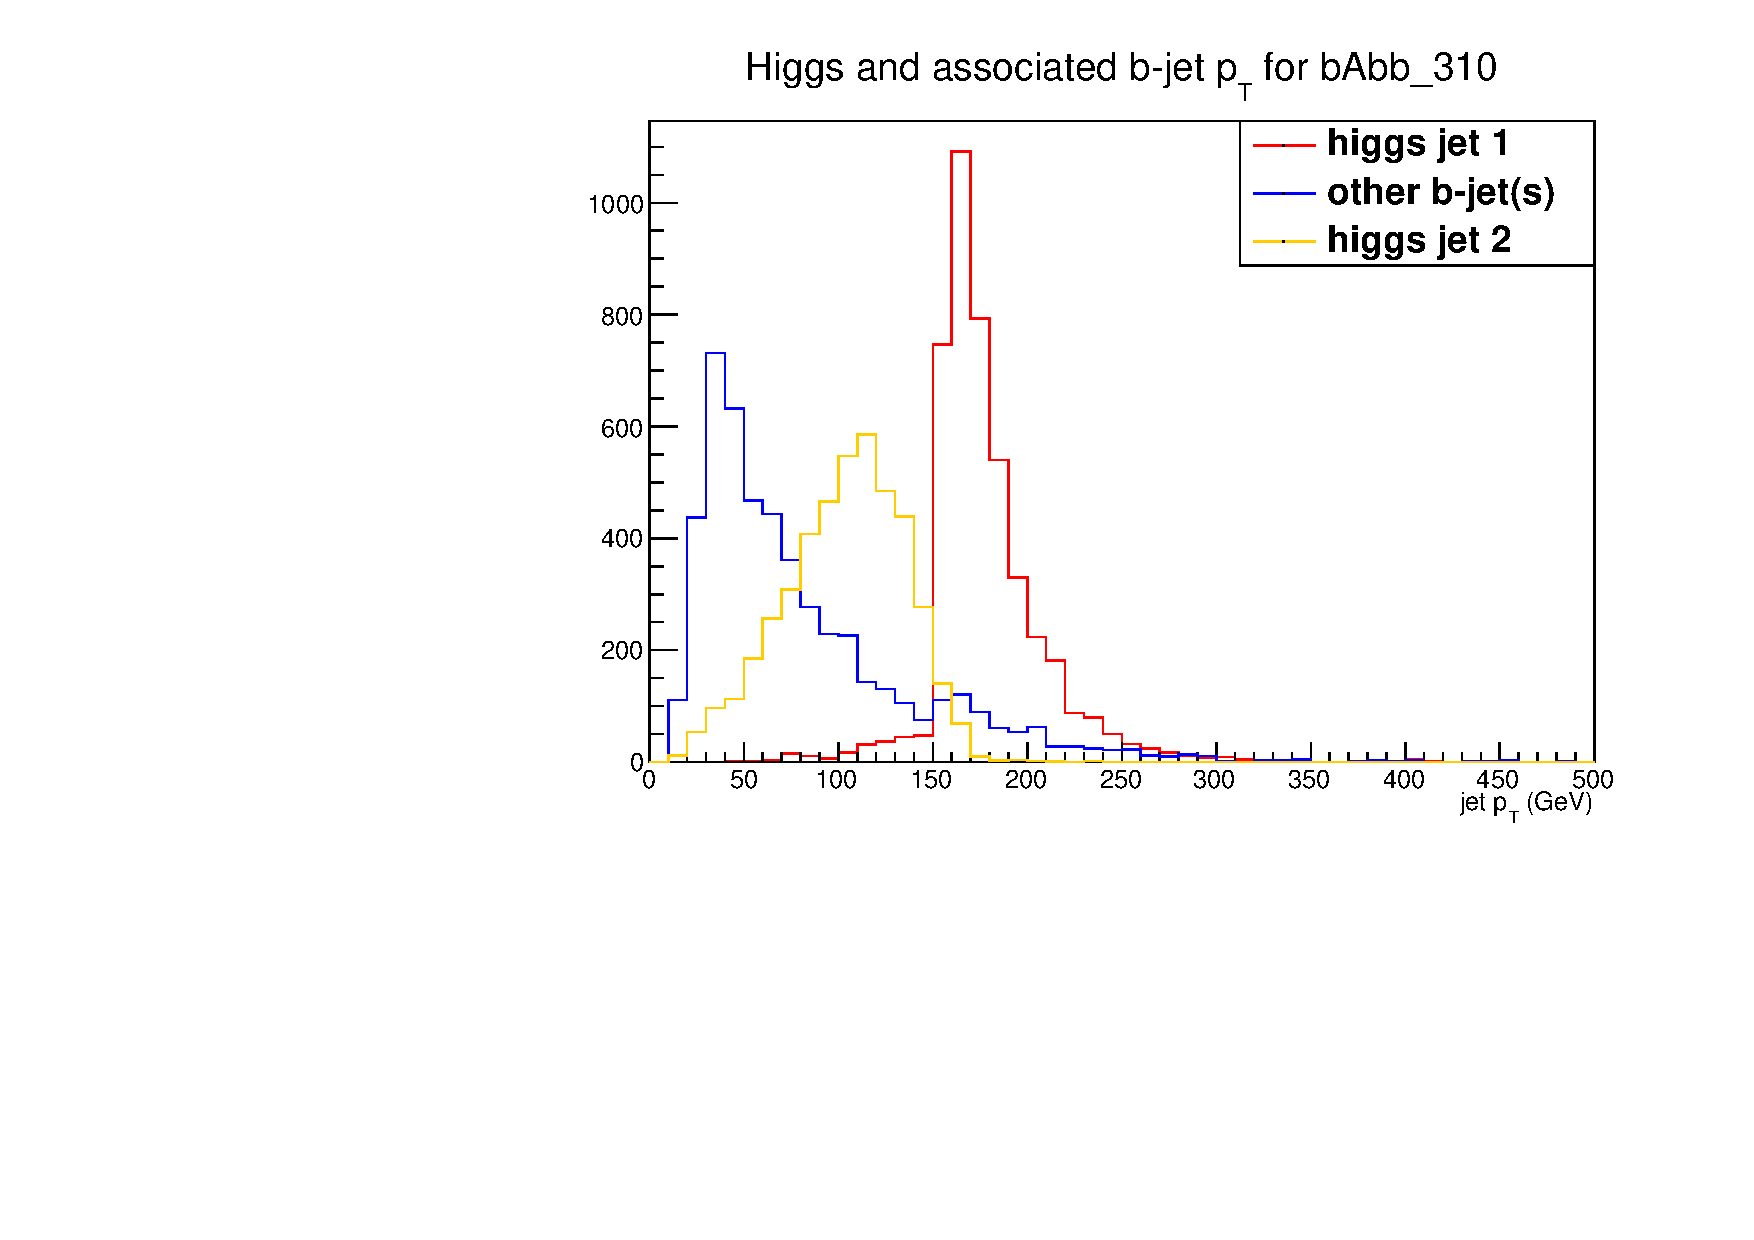
\includegraphics[width=0.3\textwidth]{SignalKin/jet_pt_compare_bAbb_310.pdf}
    \newline
    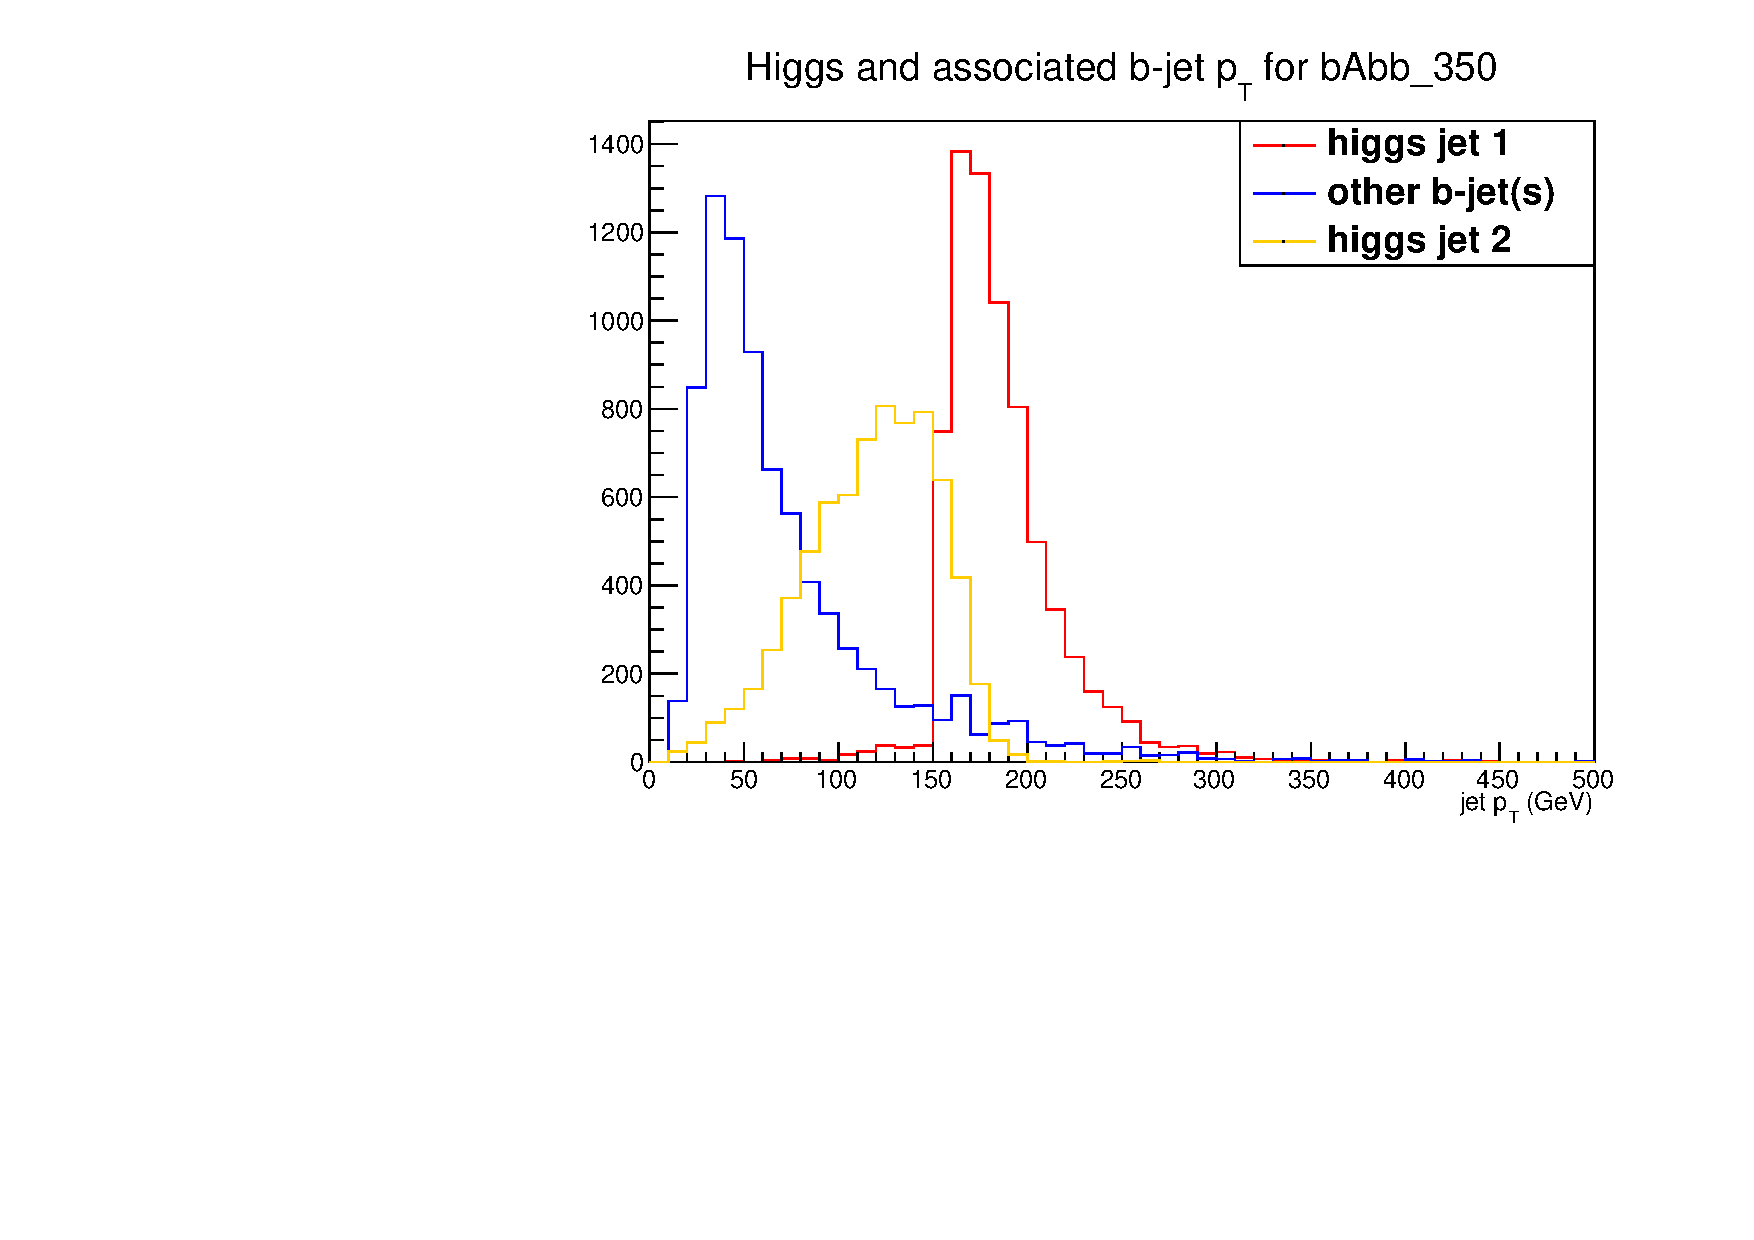
\includegraphics[width=0.3\textwidth]{SignalKin/jet_pt_compare_bAbb_350.pdf}
    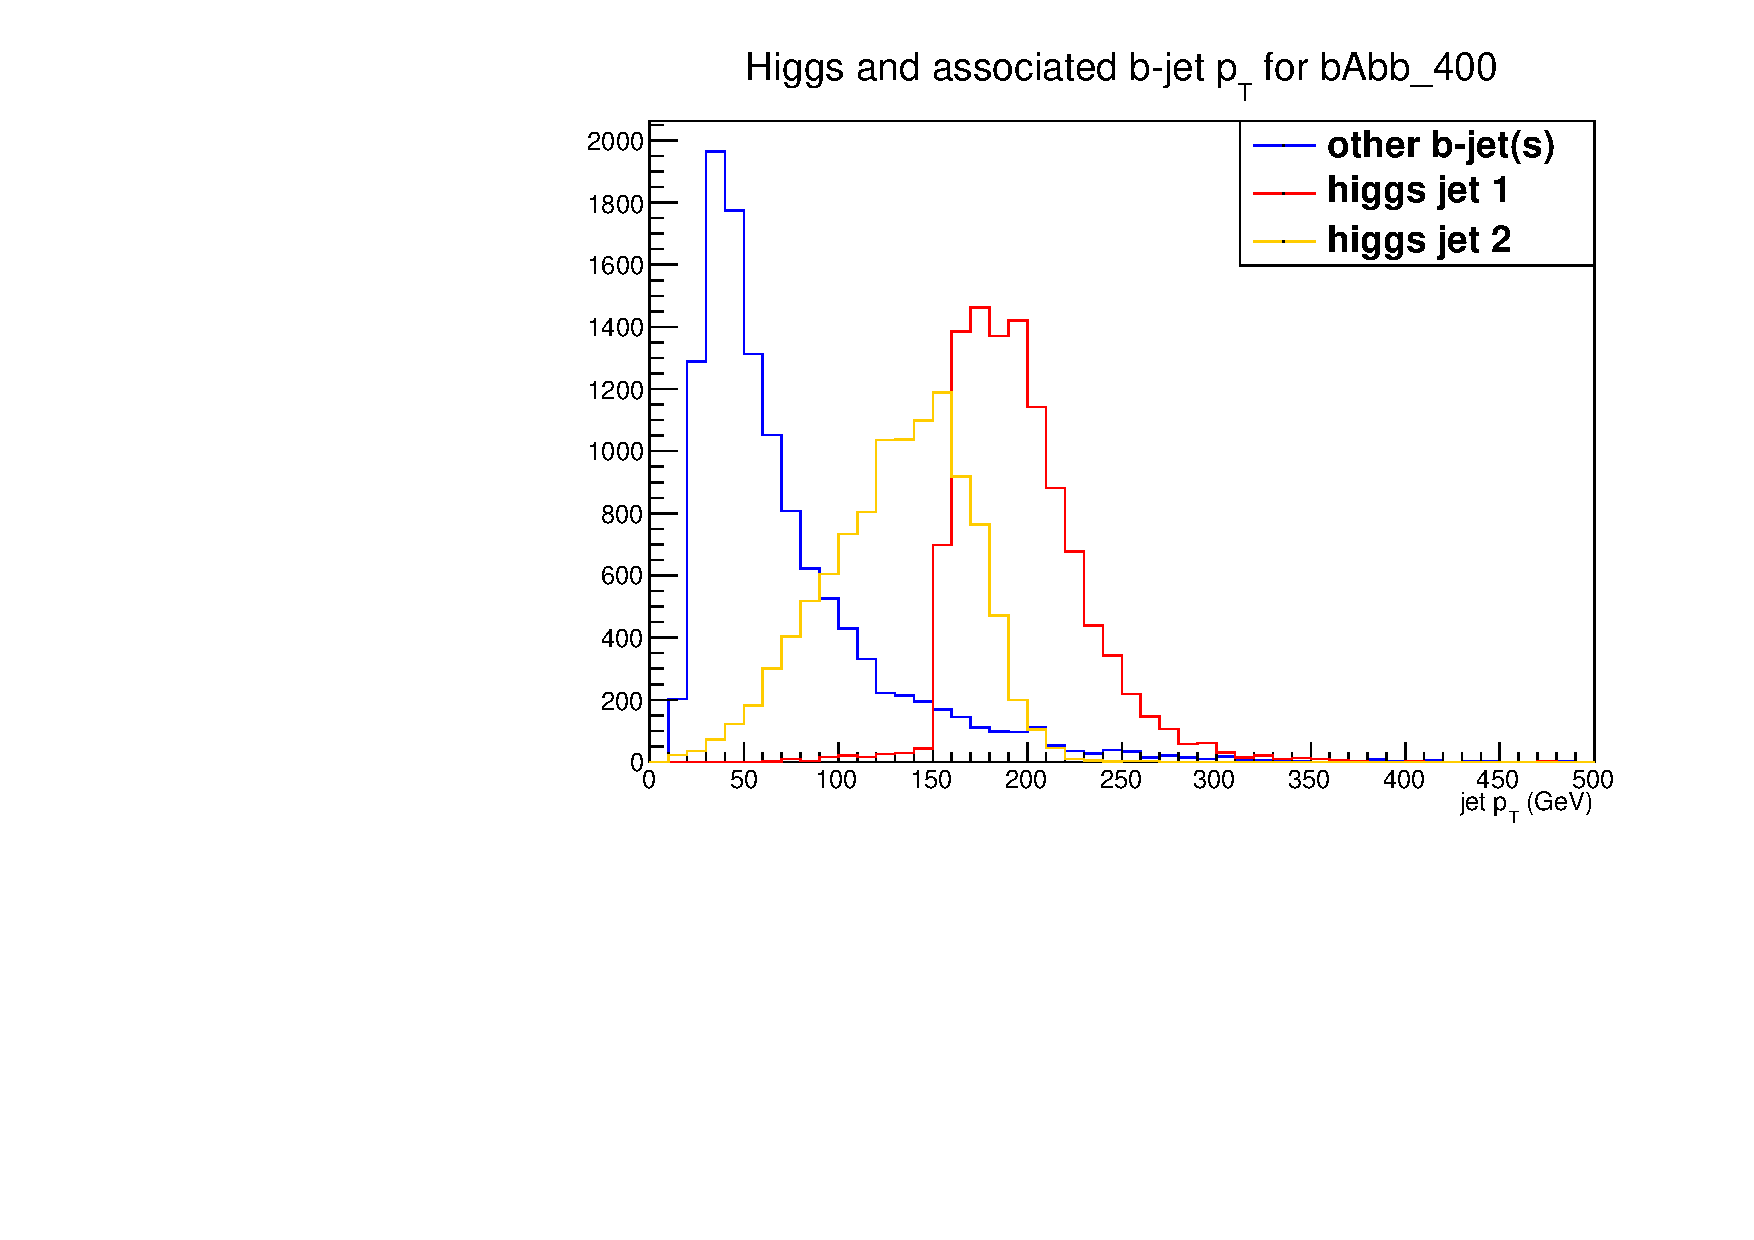
\includegraphics[width=0.3\textwidth]{SignalKin/jet_pt_compare_bAbb_400.pdf}
    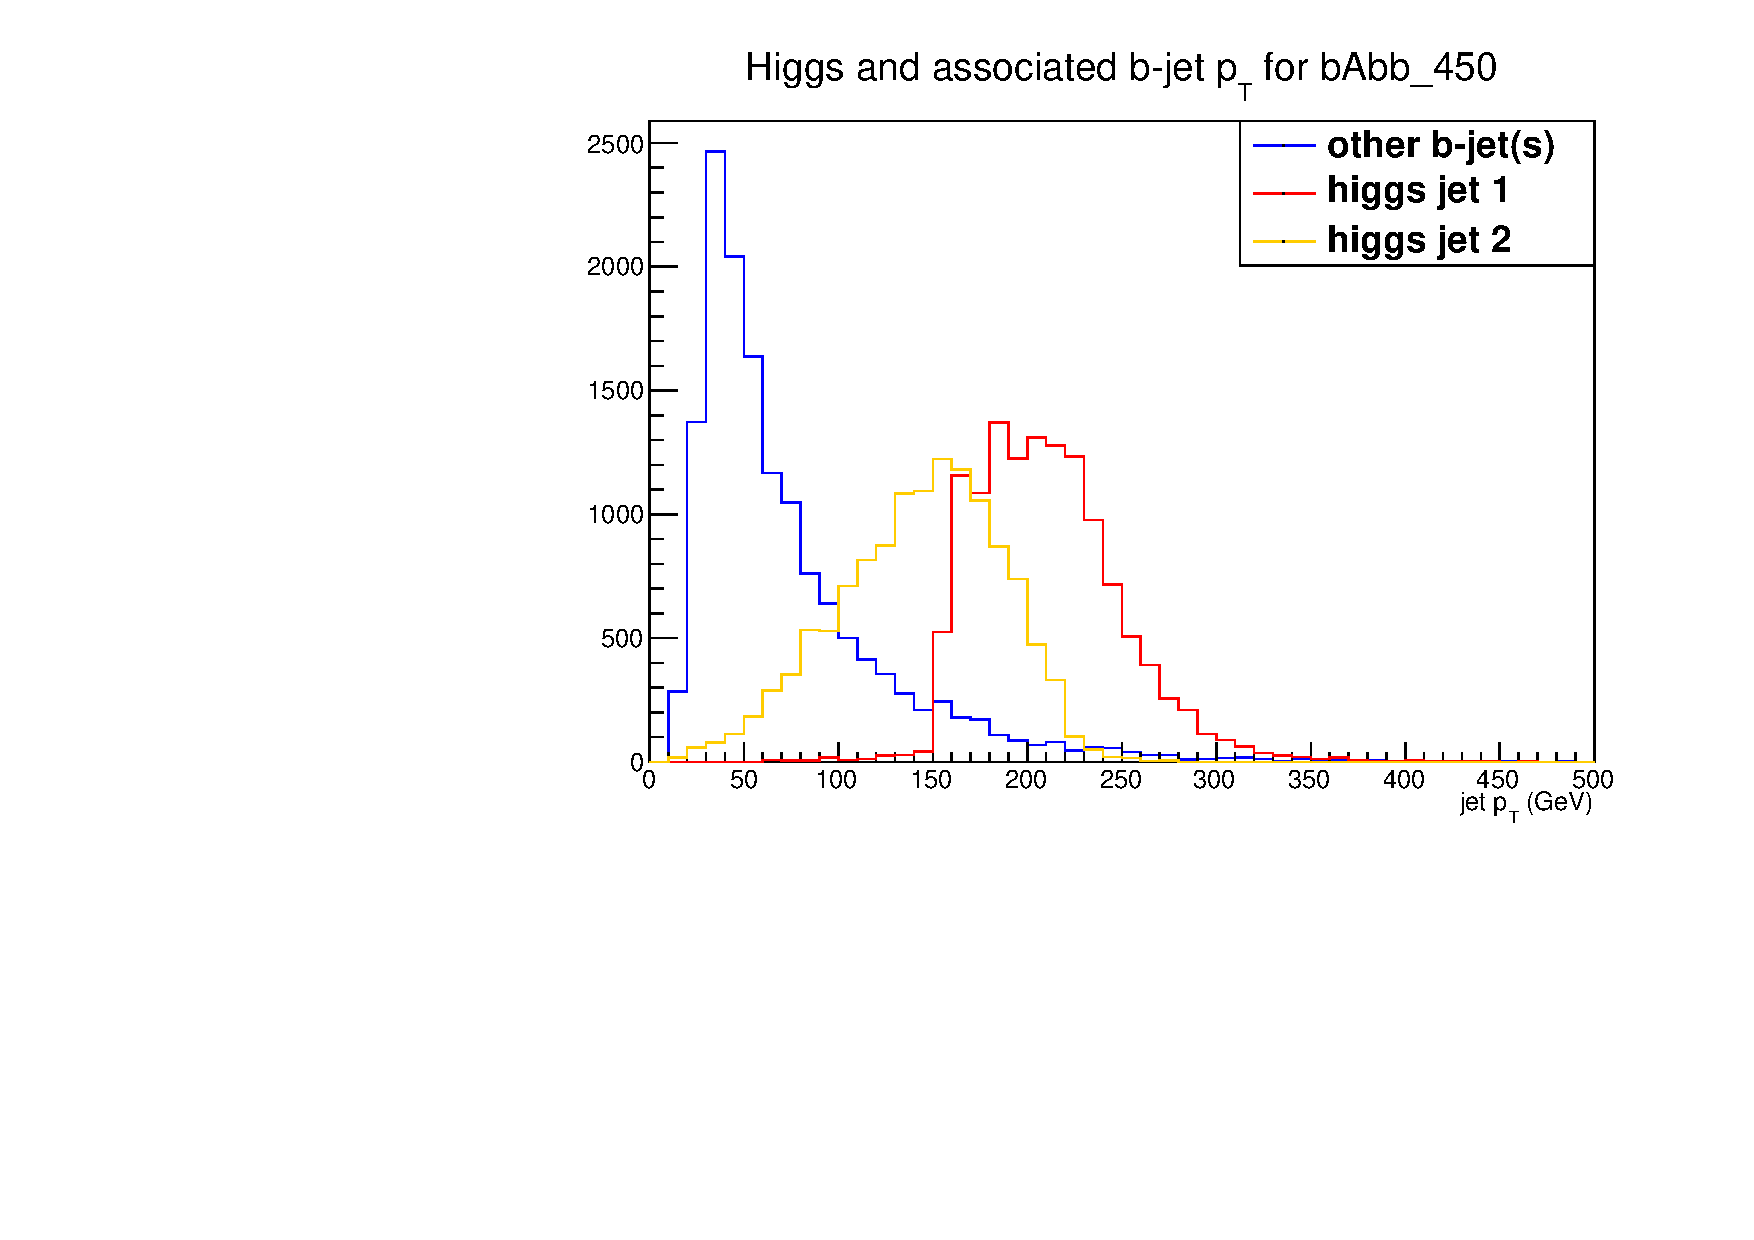
\includegraphics[width=0.3\textwidth]{SignalKin/jet_pt_compare_bAbb_450.pdf}
    \newline
    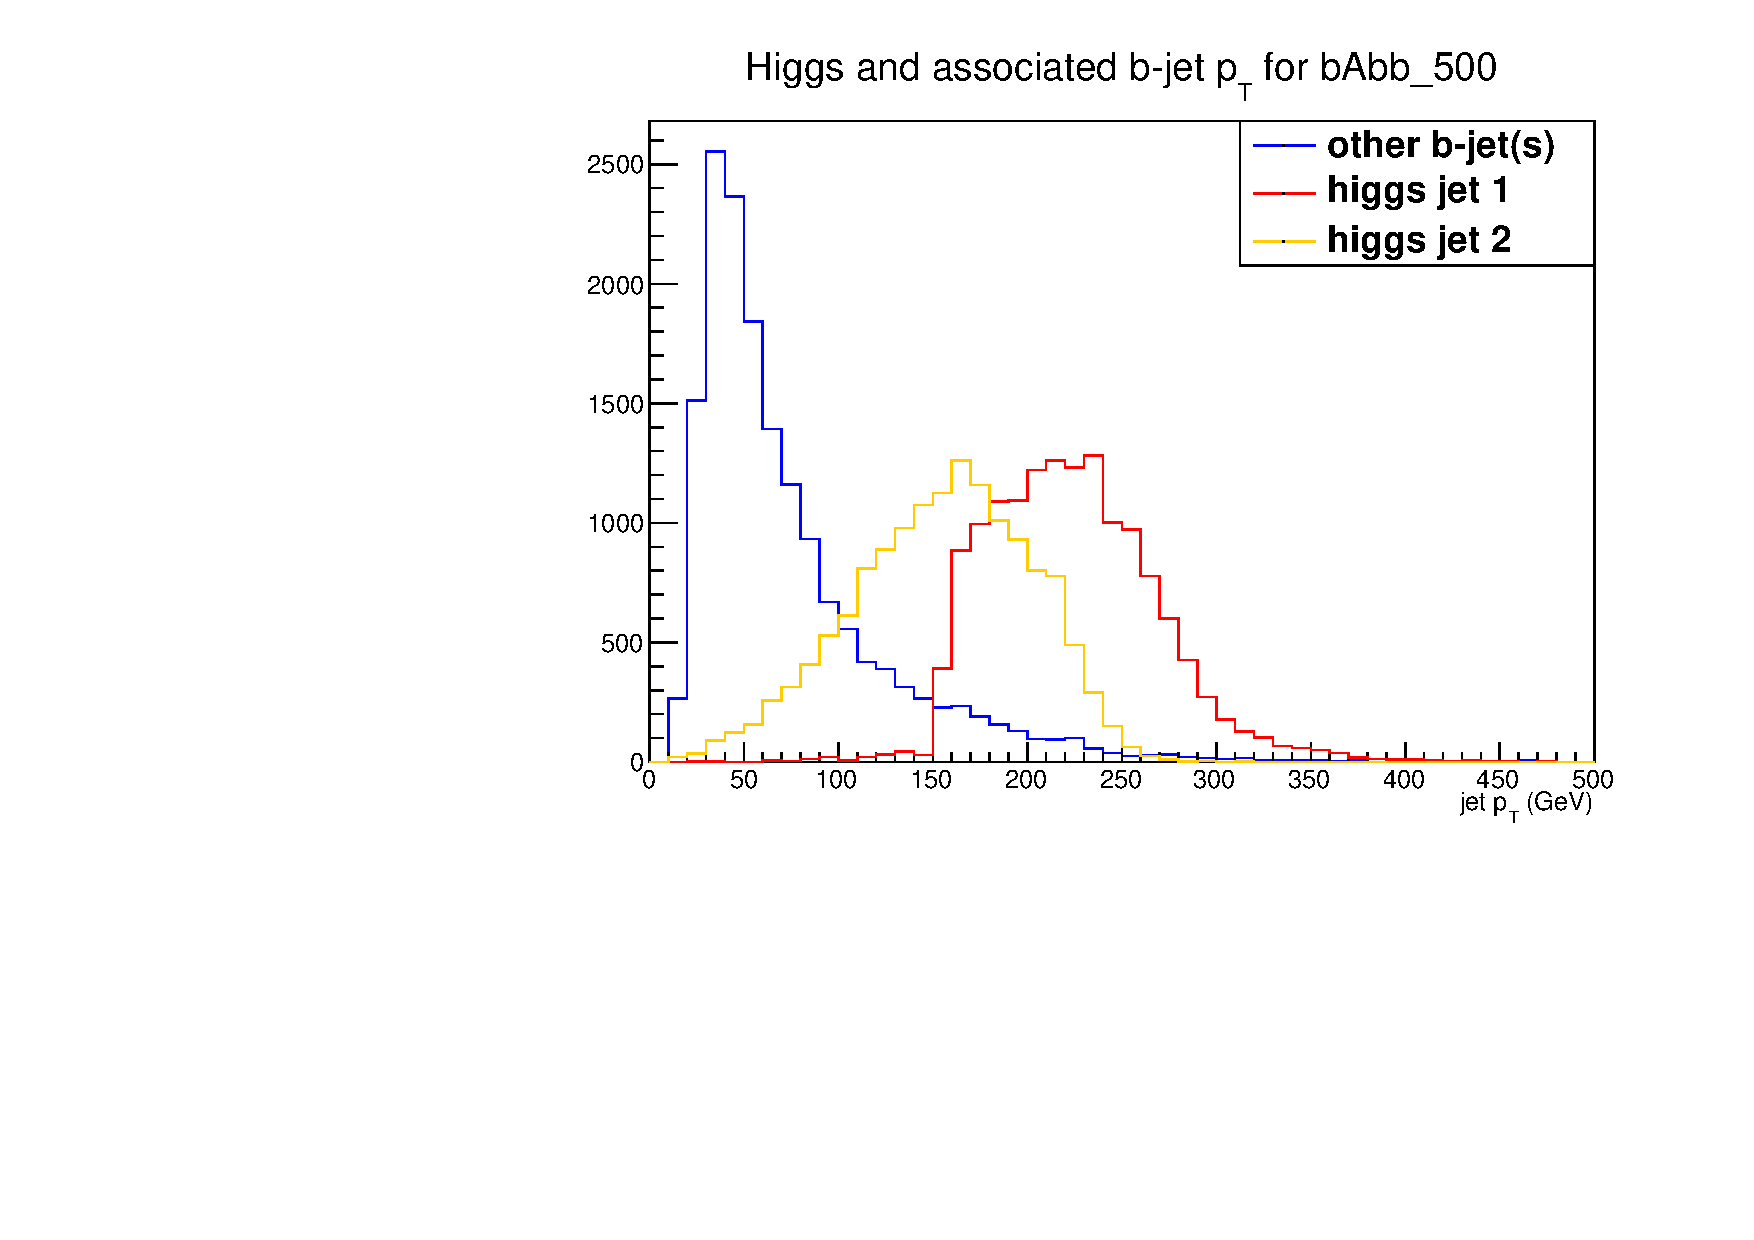
\includegraphics[width=0.3\textwidth]{SignalKin/jet_pt_compare_bAbb_500.pdf}
    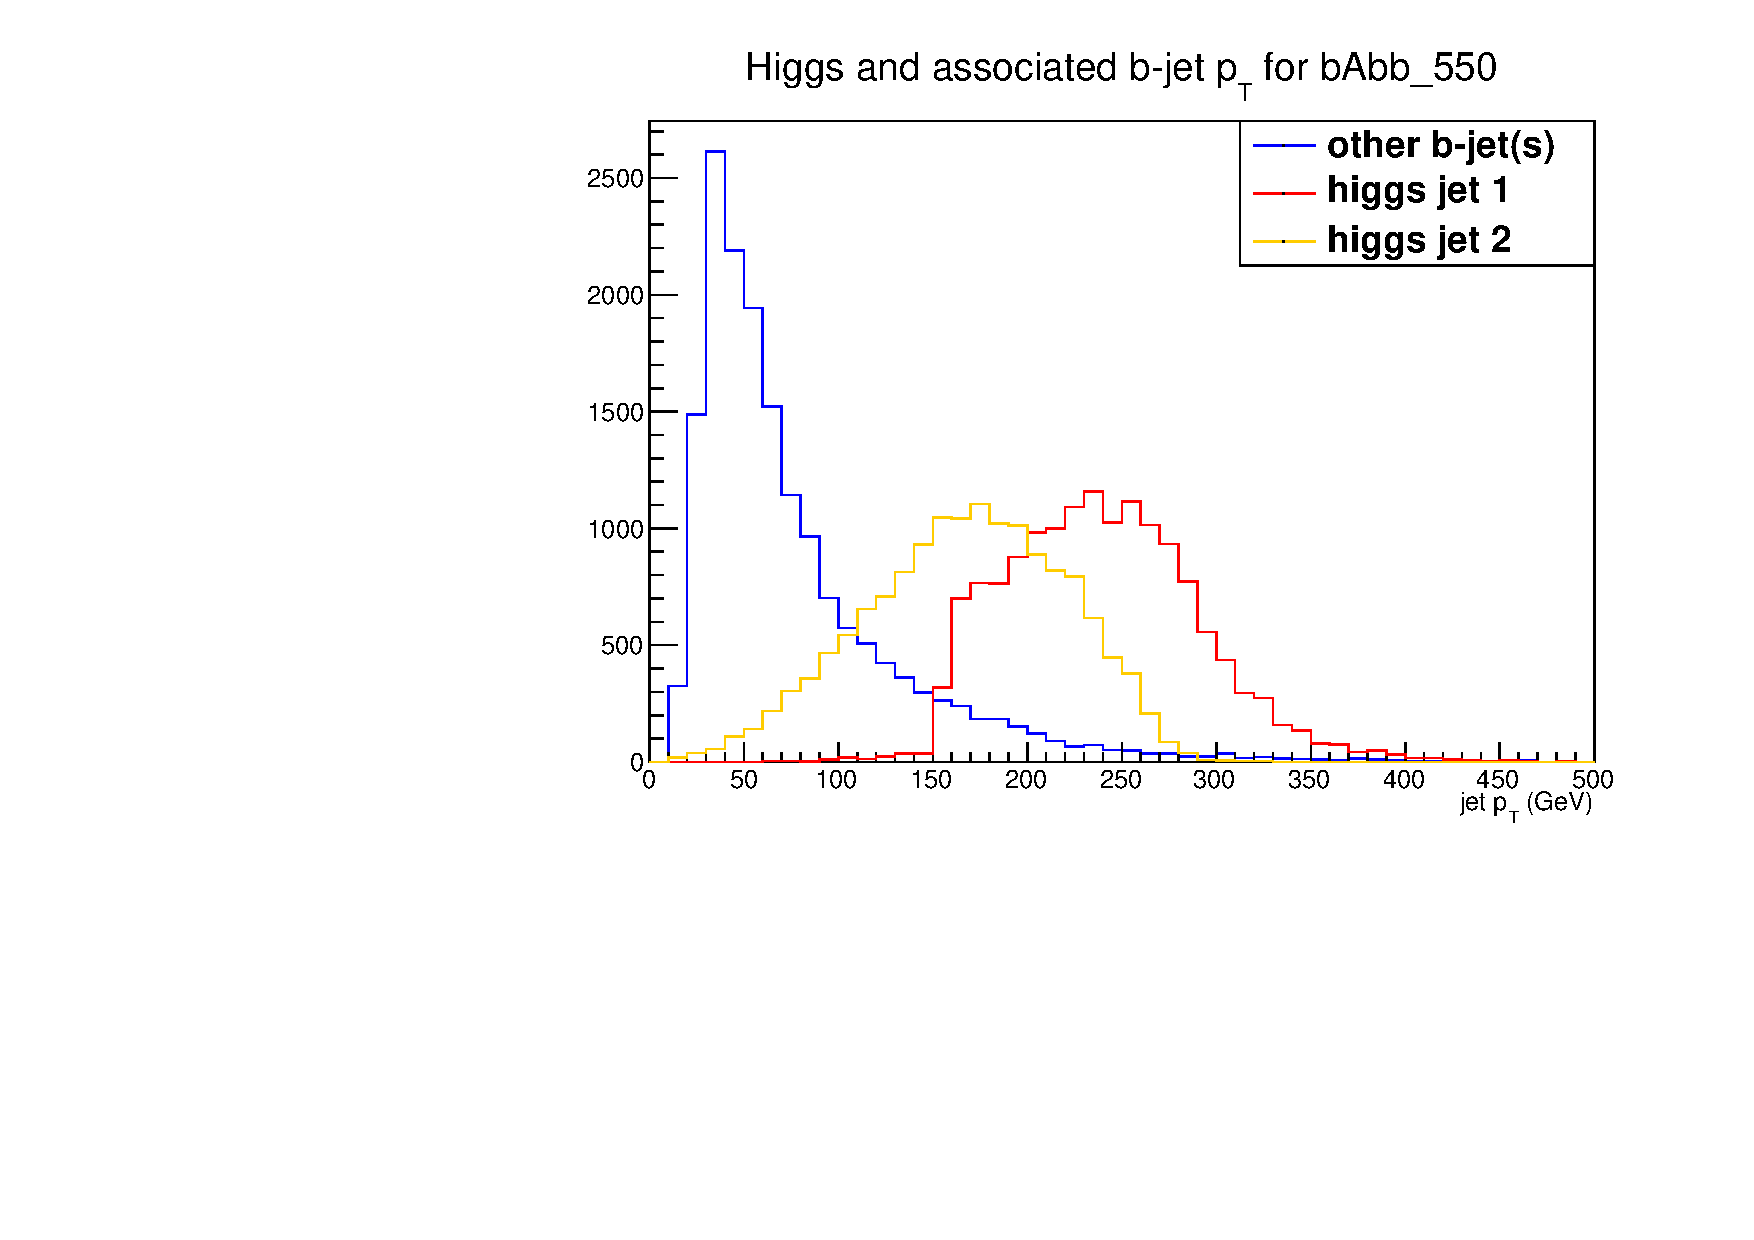
\includegraphics[width=0.3\textwidth]{SignalKin/jet_pt_compare_bAbb_550.pdf}
    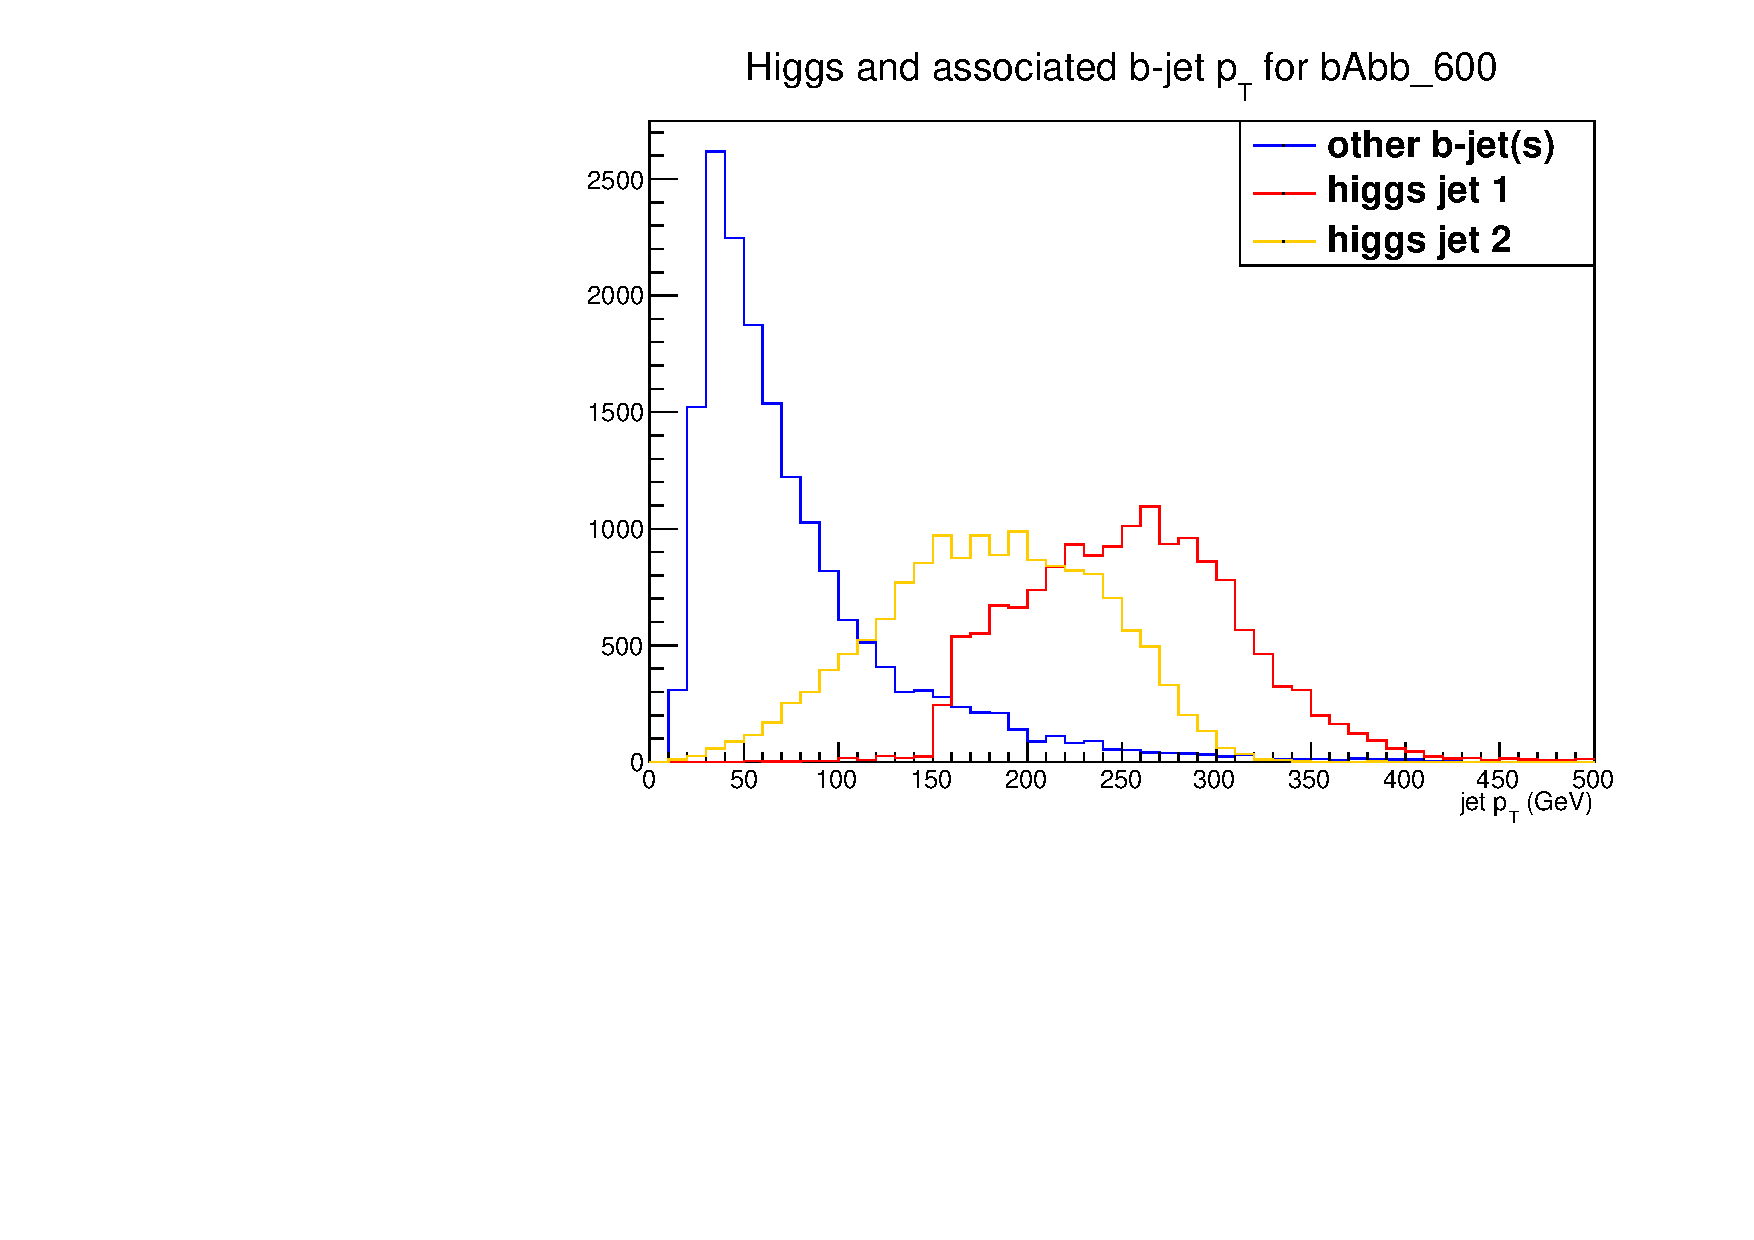
\includegraphics[width=0.3\textwidth]{SignalKin/jet_pt_compare_bAbb_600.pdf}
    \newline
    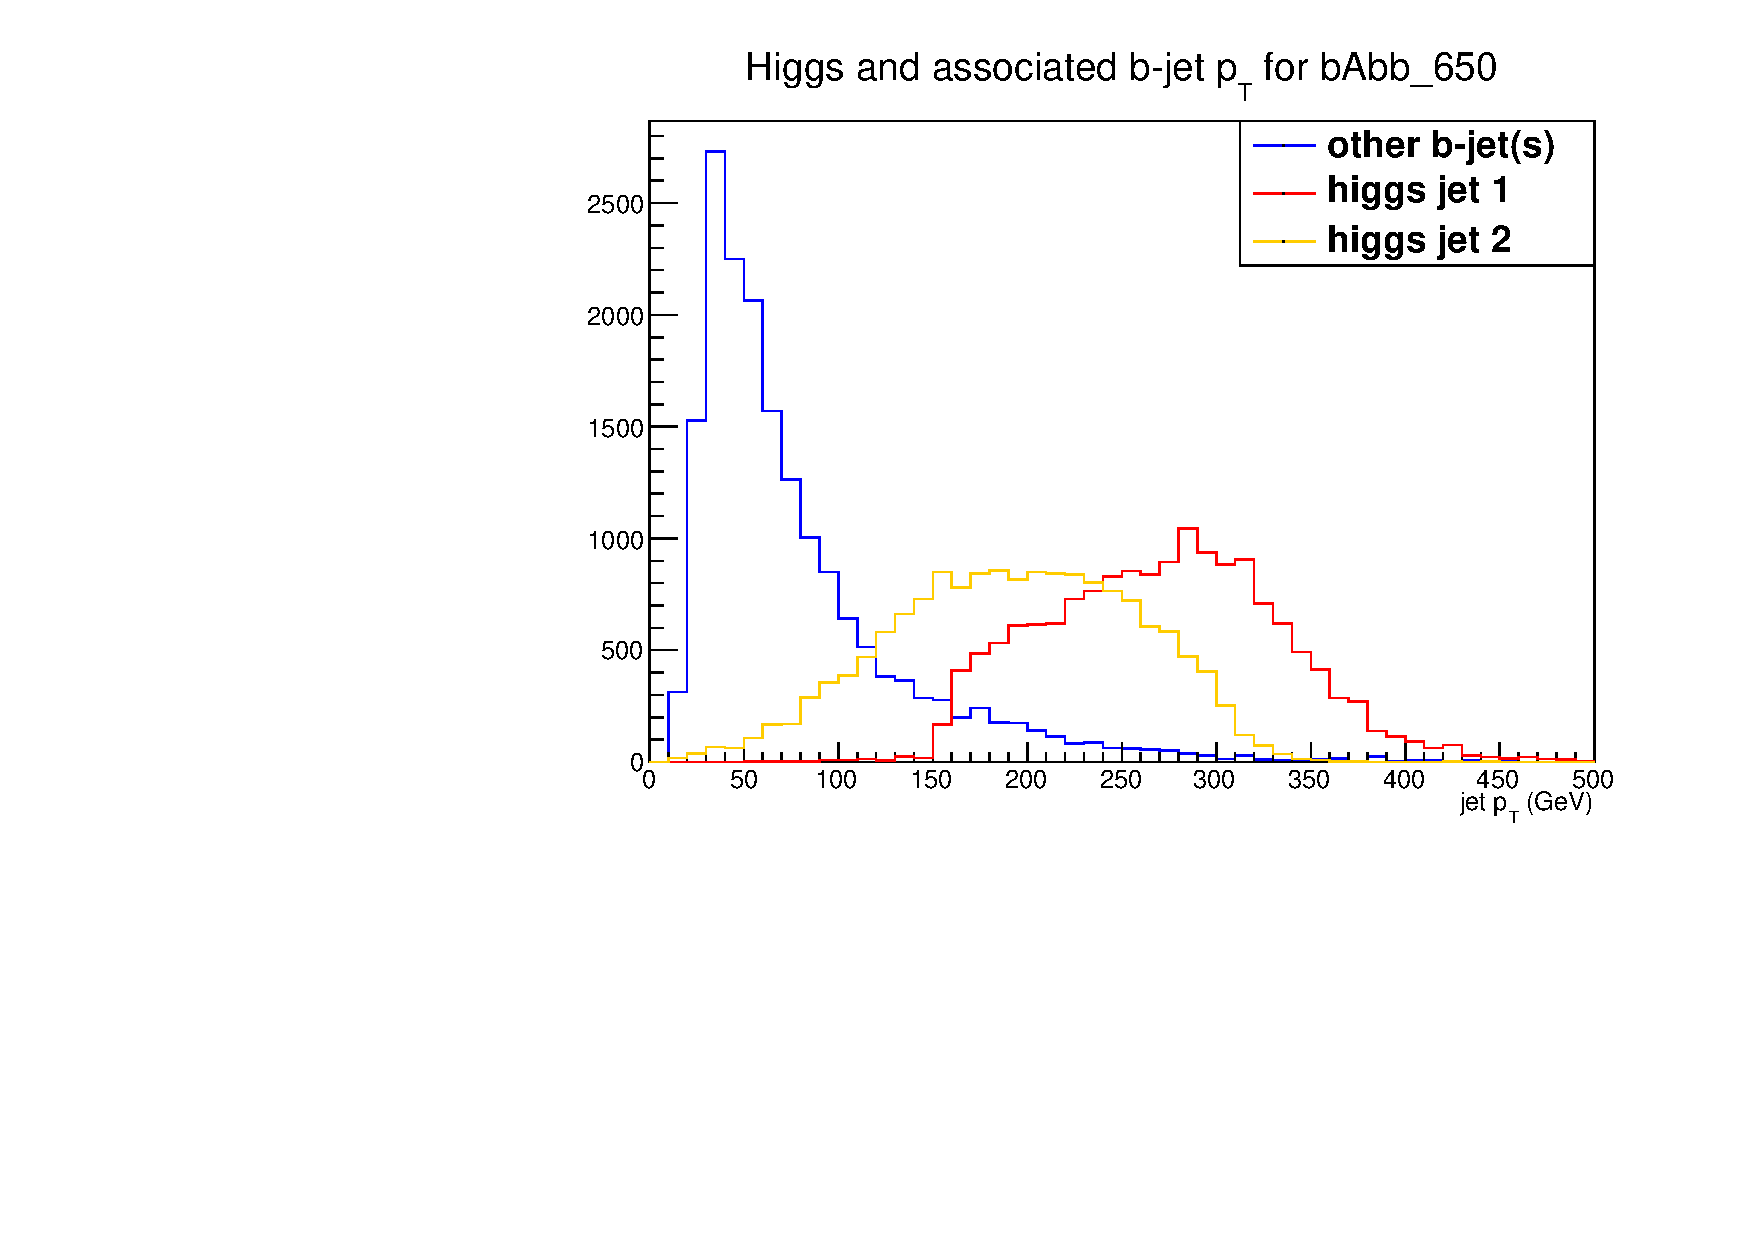
\includegraphics[width=0.3\textwidth]{SignalKin/jet_pt_compare_bAbb_650.pdf}
    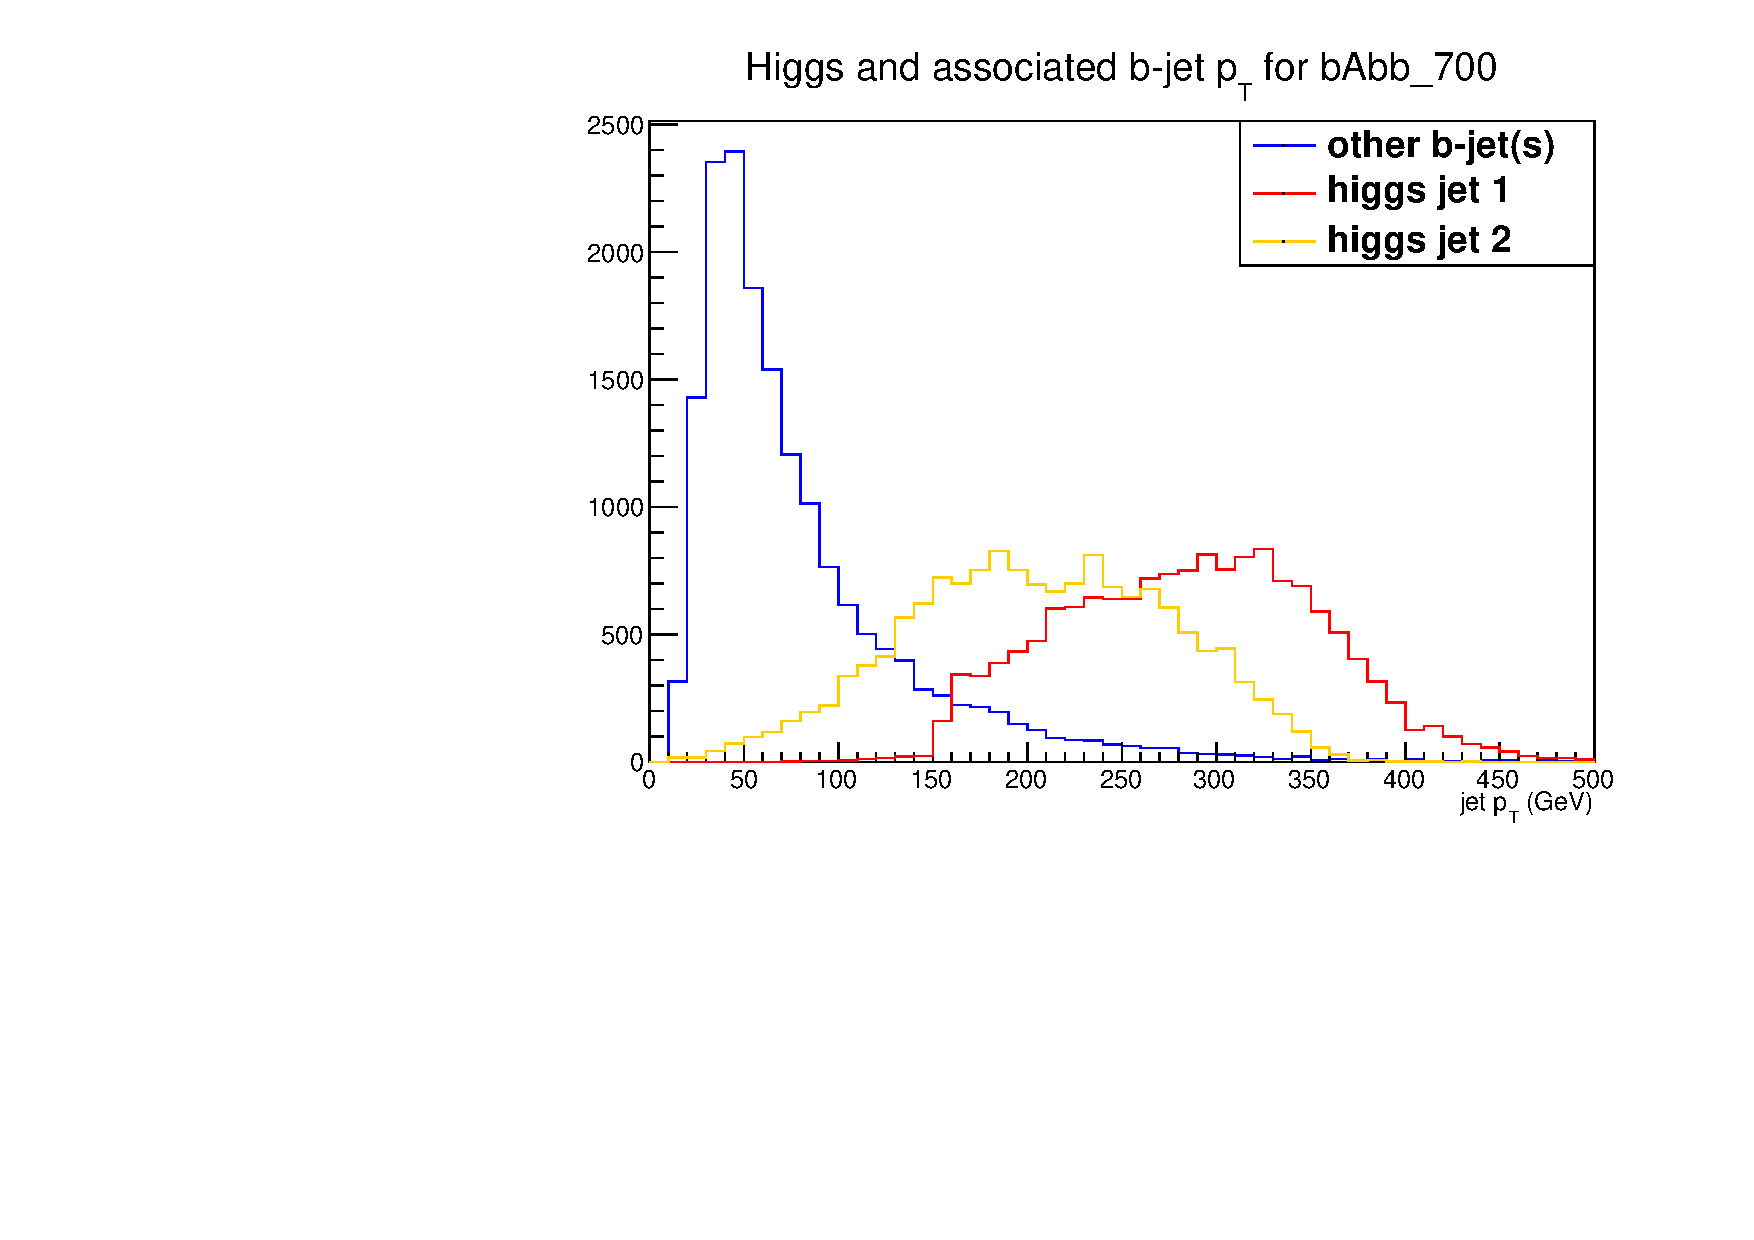
\includegraphics[width=0.3\textwidth]{SignalKin/jet_pt_compare_bAbb_700.pdf}
    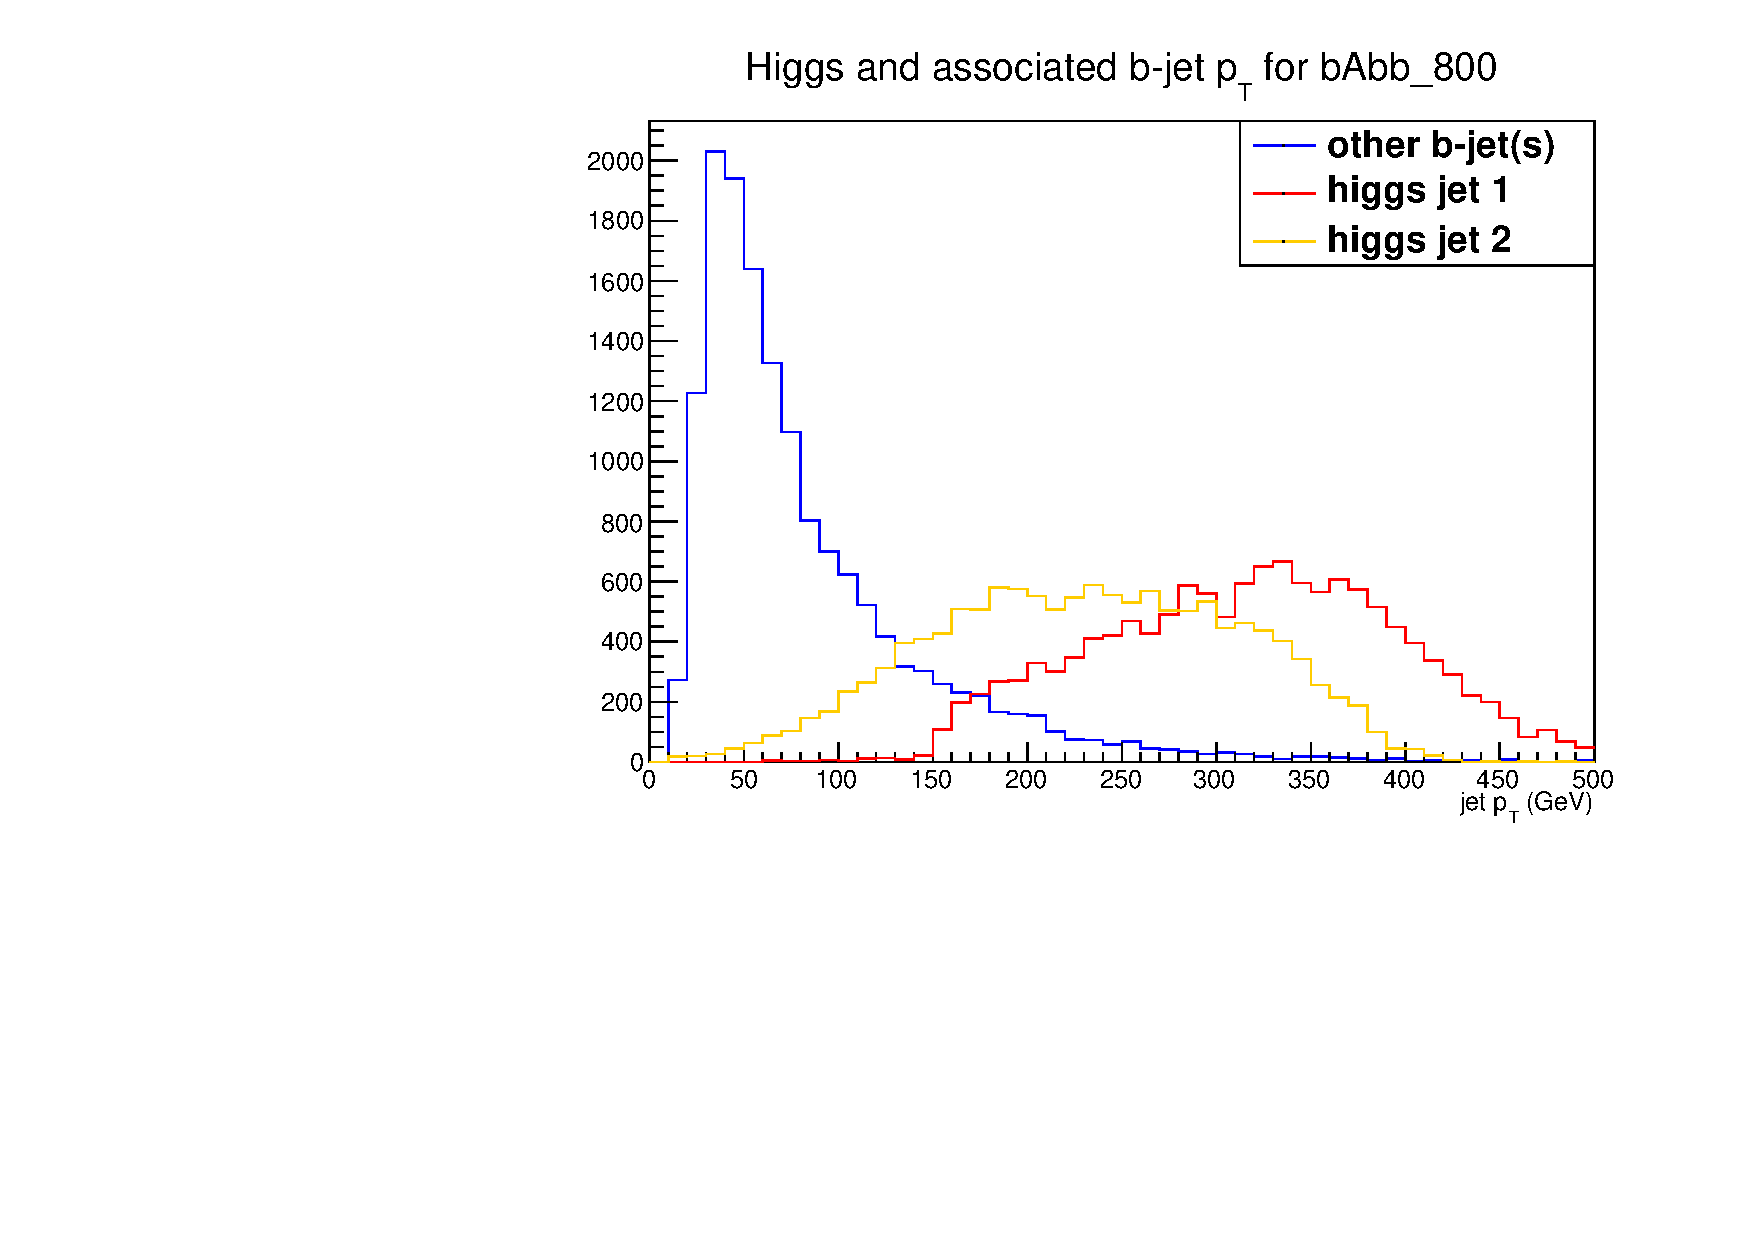
\includegraphics[width=0.3\textwidth]{SignalKin/jet_pt_compare_bAbb_800.pdf}
    \caption{The \pt of the two jets from the Higgs (classified as ``first'' and ``second'' based
    on which one has more \pt in the event), and all other $b$-tagged jet(s) in the event.
    The peaks at about 155 GeV and 55 GeV is a result of the trigger turn-on points and
    associated cut(s).  \label{fig:pt_higgs_and_associated_jets}}
\end{figure}
%----------------------------------------------

As it turns out, the presence of additional non-$b$ jets can have a significant 
effect in signal.  Since the hard scatter has only $b$-jets in the final state, the
extra jet(s) must come from other sources like initial state radiation (ISR) or 
final state radiation (FSR).  This can smear out the signal, as explained in more detail
in Section~\ref{sec:mass_res}, and combating the effects became a significant part of the
analysis.


\section{Signal Jet Combinatorics}
\label{sec:combinatorics}
An important point when trying to reconstruct the Higgs is which 2 $b$-tagged jets (of the
three available) should be used in reconstruction.  If the associated $b$-jet is accidentally
selected, then the Higgs will be mis-reconstructed and the sensitivity will suffer.  At the same time,
since the mass of the Higgs is not known, tools like a kinematic fit are not available to
help with the combinatorics.  In Figure~\ref{fig:combinatorics}, we use the MC truth
information in the signal MC to plot how often the Higgs decays to various pairs of jets
within the event; we find that especially for masses above 350 GeV or so it usually decays to
the leading and second $b$-tagged jets in the event (with about a 70\% probability).
    
\begin{figure}[hbt]
  \center
  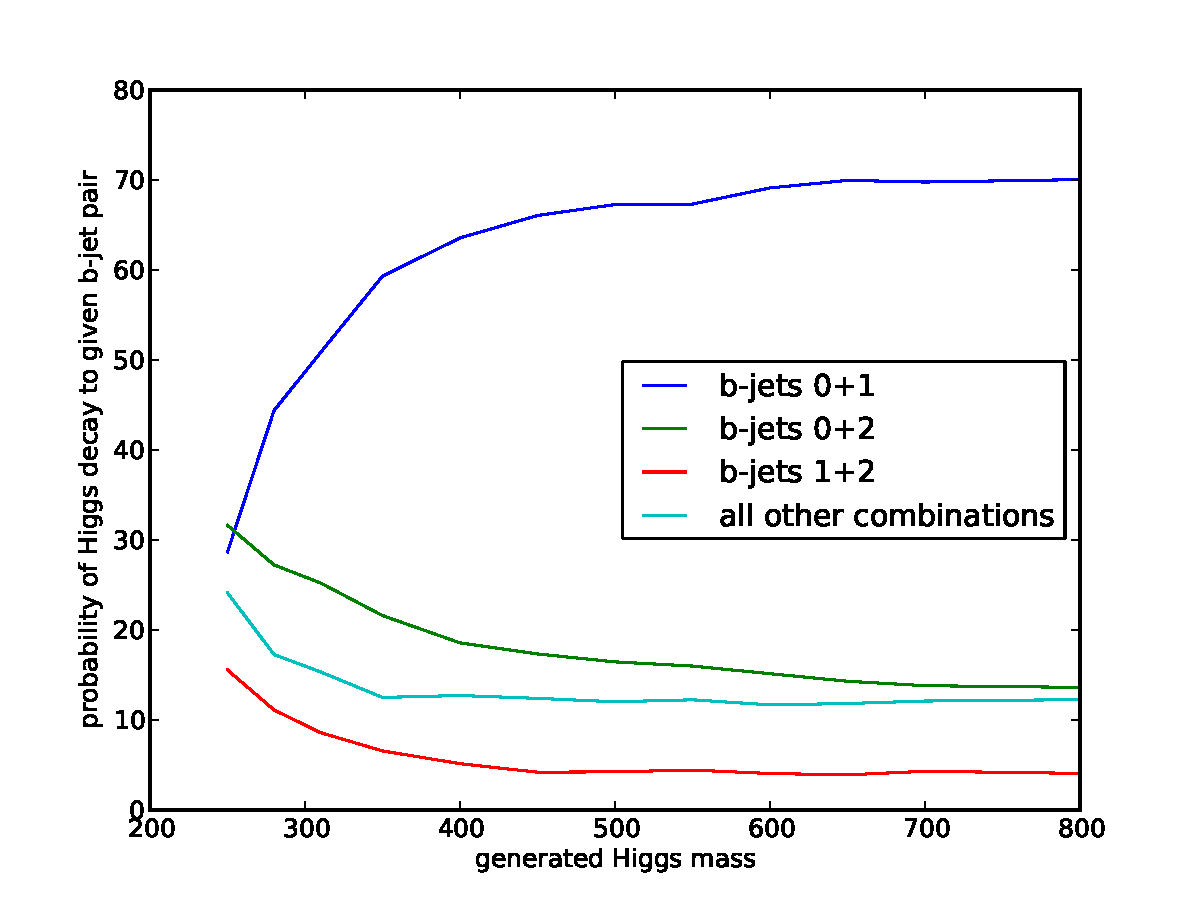
\includegraphics[width=0.78\linewidth]{SignalKin/combinatorics.pdf}
  \caption{The percentage probability of the Higgs decaying to a given pair of $b$-tagged jets in signal MC,
    as a function of the generated Higgs mass.  The assumption being checked is that the majority of
    the time, the Higgs decays to the leading two $b$-tagged jets (blue line), so that reconstructing with these jets
    will yield the correct combinatorics.  That assumption is correct 60-70\% of the time for $m_A>$350 GeV,
    with the remaining 30-40\% of events being spread out over many other combinations of jets.
    \label{fig:combinatorics}}
\end{figure}
                
\begin{figure}
  \centering
    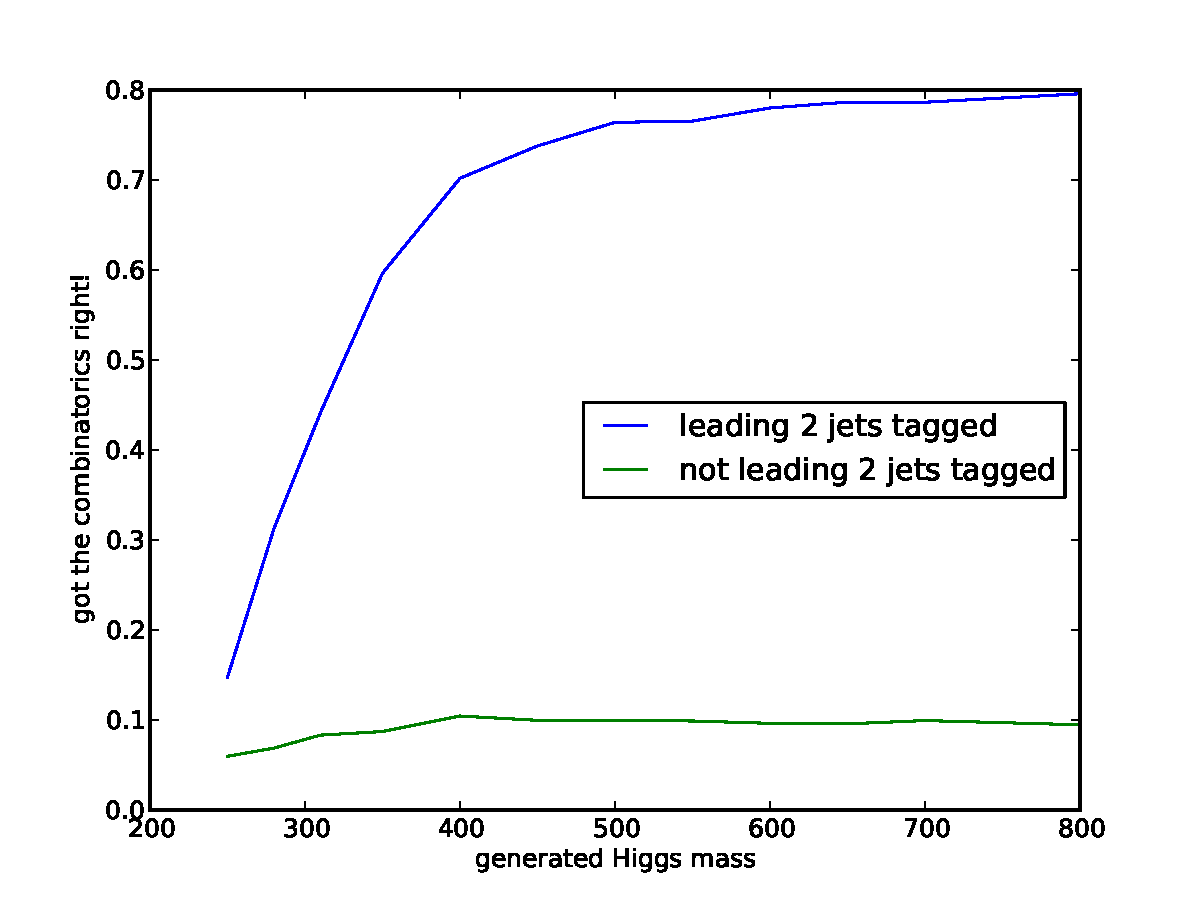
\includegraphics[width=0.78\linewidth]{SignalKin/combinatorics_success.pdf}
    \label{fig:combinatorics_success}
    \caption{After making the requirement that the leading two jets in the event are $b$-tagged,
    the signal MC can be split into events that pass this requirement and those events that fail.
    For each sample, we ask how often the Higgs decays to the leading two $b$-jets in the event,
    or in other words, how likely it is to get the combinatorics of the Higgs reconstruction correct.
    The combinatorics for the events passing the requirement are correct about 80\% of the time for
    high m$_H$, while for events failing the requirement the combinatorics success rate is only about 10\%.}
\end{figure}
                                                                                                                                                                 
                                                                                                                                    
If we require only that the leading 2 $b$-tagged jets be used in reconstruction, there can                                          
still be events in our sample where the leading 2 $b$-tagged jets in the event are not                                              
the leading 2 jets overall--for example, there can be a very hard light jet, and the $b$-tagged                                     
jets are the second and third jets in $p_T$.  When we introduce a cut that eliminates these events,                                 
by requiring that the leading 2 jets in the event be $b$-tagged, both the signal to background                                      
ratio improves (this cut is about 25\% efficient in background, and over 90\% efficient                                             
in signal) and the mass resolution is improved in signal as the events that rejected have                                           
hard FSR present and the reconstructed $m_{bb}$ is far from the generated $m_A$.    




\section{Mass Resolution}
\label{sec:mass_res}
%Once the trigger and all the analysis cuts have been applied, we take the leading 2 jets in the 
%event (which are also the leading 2 $b$-tagged jets, since we place a cut requiring 
%that the leading 2 jets in the event be $b$-tagged) and reconstruct their combined invariant mass
%--if they came from a decaying particle, the reconstructed mass should be the mass of the parent particle
%.  On the other hand, if the leading 2 jets come from continuum QCD processes, there should be 
%no resonance present, so we look for the presence of a resonance peak on top of a decaying power
%-law background.


A consistent refrain throughout this analysis is the challenge of poor mass resolution when reconstructing
the signal, especially in the low-mass tail for high values of $m_A$. The 
issue is important because a poorly-reconstructed (very wide)
signal peak can easily be confused with a background normalization error, which makes the analysis less
sensitive to small signals. This section will summarize the efforts to make the mass resolution as good
as possible; some tactics did produce an improvement while others did not.  In brief, the tactics
attempted include the following:

\begin{itemize}
    \item require that the leading 2 jets in the event be b-tagged (improved resolution)
    \item when b-tagged jets have one or more jets nearby, include those jets in the mbb reconstruction (does
not improve resolution)
    \item when a hard ($>$80 GeV) untagged jet is present in an event, include it in the mbb reconstruction
(does not improve resolution)
\end{itemize}


The problem is significantly worse at higher masses;
to some extent, this is inevitable because the inherent width of the Higgs resonance increases with $m_A$
(quantification of this effect can be found in Figure~\ref{fig:width}). However, the inherent width goes up to about 12
GeV (at $m_A$=800 GeV), while the width of the reconstructed mass peak goes up to several hundred GeV.
With this in mind, it’s clear that other effects drive the mass resolution.  The following sections, 
and the tactics documented in them that attempt to recover lost mass resolution, focus mainly 
on two hypotheses: that the lost mass resolution arises from final state radiation (FSR), and/or
that it arises from incorrectly picking the jets when reconstructing (combinatorics). 




\subsection{Mass Resolution Improvement after Requiring that Leading Two Jets be $b$-Tagged}
The first strategy for recovering mass resolution is to require, as part of the cut flow,
that the leading 2 jets in the event be $b$-tagged.  Before this cut is applied, it is
possible to have signal events in which there is hard ISR or FSR (light jet radiation),
and/or $b$-jets from the signal process that are high-$p_T$ but do not pass the $b$-tagging.
The price of this cut is a loss in signal efficiency, which varies by $m_A$ but can be 
seen in Figure~\ref{fig:combinatorics} to be about 30-40\% above $m_A$=350 GeV or so.
However, Figure~\ref{fig:background_eff_cutflow} shows that the background also drops, 
by a higher amount that varies based on the exact background in question, so that the net 
effect on signal/background for this cut is neutral or favorable.
 

Quantifying the effect of this cut on the mass resolution is a little tricky because of the
$m_{bb}$ shape in signal, which is highly asymmetric.  In order to make some progress, though,
we define the ``left'' and ``right'' shoulders of the distribution, where the left shoulder
corresponds to the low-mass side of the $m_{bb}$ distribution, where the reconstructed mass 
is below the peak for a given signal mass point,
and the right shoulder is the part of the distribution above the peak.  Then we can define
a threshold corresponding to 20\% of the peak height, and ask for the left-shoulder and right-shoulder
windows where the distribution is above the threshold.  The right shoulder is much narrower,
and any events in the high-mass tail (above the generated value for $m_A$) arise from 
combinatorial mis-reconstructions.  The left shoulder, where FSR and combinatorics are
at play, is significantly wider but improved by 40\% (at $m_A$=800 GeV) to 300\% (at $m_A$=250 GeV)
once we require that the leading 2 jets in the event be $b$-tagged.  The widths of the shoulders
for all mass points, before and after this cut is applied, can be seen in Table~\ref{tab:signal_mass_RMS_compare}.
%The plots in Figure 39 and Figure 40 show the ect on the invariant mass distribution.
% In order to quantify the mass resolution ect, we define the “left” and “right” shoulders of the mbb
% distribution, which are respectively the portion of the mbb distribution that are below and above the peak.
% go into further detail on the signal shape in Section 6.2; but in Table~\ref{tab:signal_mass_RMS_compare} the RMS of especially the left
% shoulder before and after requiring b-tags on the leading 2 jets quantitatively shows the mass resolution
% improvement.



%----------------------------------------------
\begin{table}
\centering
\caption{The width of the mass distribution in the left and right shoulders of the peak,
    as explained in the text.  The left shoulder is dominated by radiation off the Higgs
    and/or the Higgs daughter jets in addition to combinatorial mis-reconstructions,
    leading to a larger RMS than the right shoulder, which
    is dominated by combinatorics only.\label{tab:signal_mass_RMS_compare}   }
  \begin{tabular}{ccccc}
     \hline \hline
     $m_A$ (GeV) & \multicolumn{2}{c}{$b$-tags on leading jets (GeV)} & \multicolumn{2}{c}{no $b$-tags on leading jets (GeV)}  \\
        & left & right & left & right \\ \hline
     250 & 13.5 & 89.2 & 36.7 & 87.7 \\
     280 & 19.2 & 68.8 & 27.5 & 71.4 \\
     310 & 19.2 & 58.3 & 31.8 & 58.1 \\
     350 & 28.3 & 34.5 & 33.9 & 36.2 \\
     400 & 33.4 & 26.1 & 45.1 & 26.5 \\
     450 & 39.5 & 25.7 & 62.2 & 25.9 \\
     500 & 48.6 & 29.3 & 81.1 & 29.8 \\
     550 & 54.9 & 31.1 & 93.1 & 33.3 \\
     600 & 73.0 & 26.0 & 117.6 & 30.5 \\
     650 & 75.4 & 31.7 & 130.8 & 31.8 \\
     700 & 75.7 & 40.3 & 143.4 & 40.7 \\
     800 & 100.9 & 36.2 & 177.4 & 36.3 \\
     \hline     \end{tabular}
\end{table}
%----------------------------------------------






\subsection{Validation of Qualitative Shape Differences}
The first question to ask is whether the high-mass mbb distributions are qualitatively lower-resolution than
the low-mass distributions–in other words, whether the ratio of the width to the generated mass changes
as a function of mass. We probe this by “normalizing” the signal MC mass, dividing each entry in the mbb
histogram by the nominal mass which was generated; for example, a signal MC event that was generated
with a Higgs mass of 350 GeV and reconstructed to have 300 GeV would be entered into the histogram
as (300/350). Repeating this normalization process for several mass points allows us to compare the
shapes for different $m_A$ values.
We find that even when the mbb distributions are renormalized, the high-mass distributions remain
wider than the low-mass distributions. That points toward FSR as a likely culprit, and in the following
sections we will detail several attempts at FSR recovery.
\begin{figure}[hbt]
  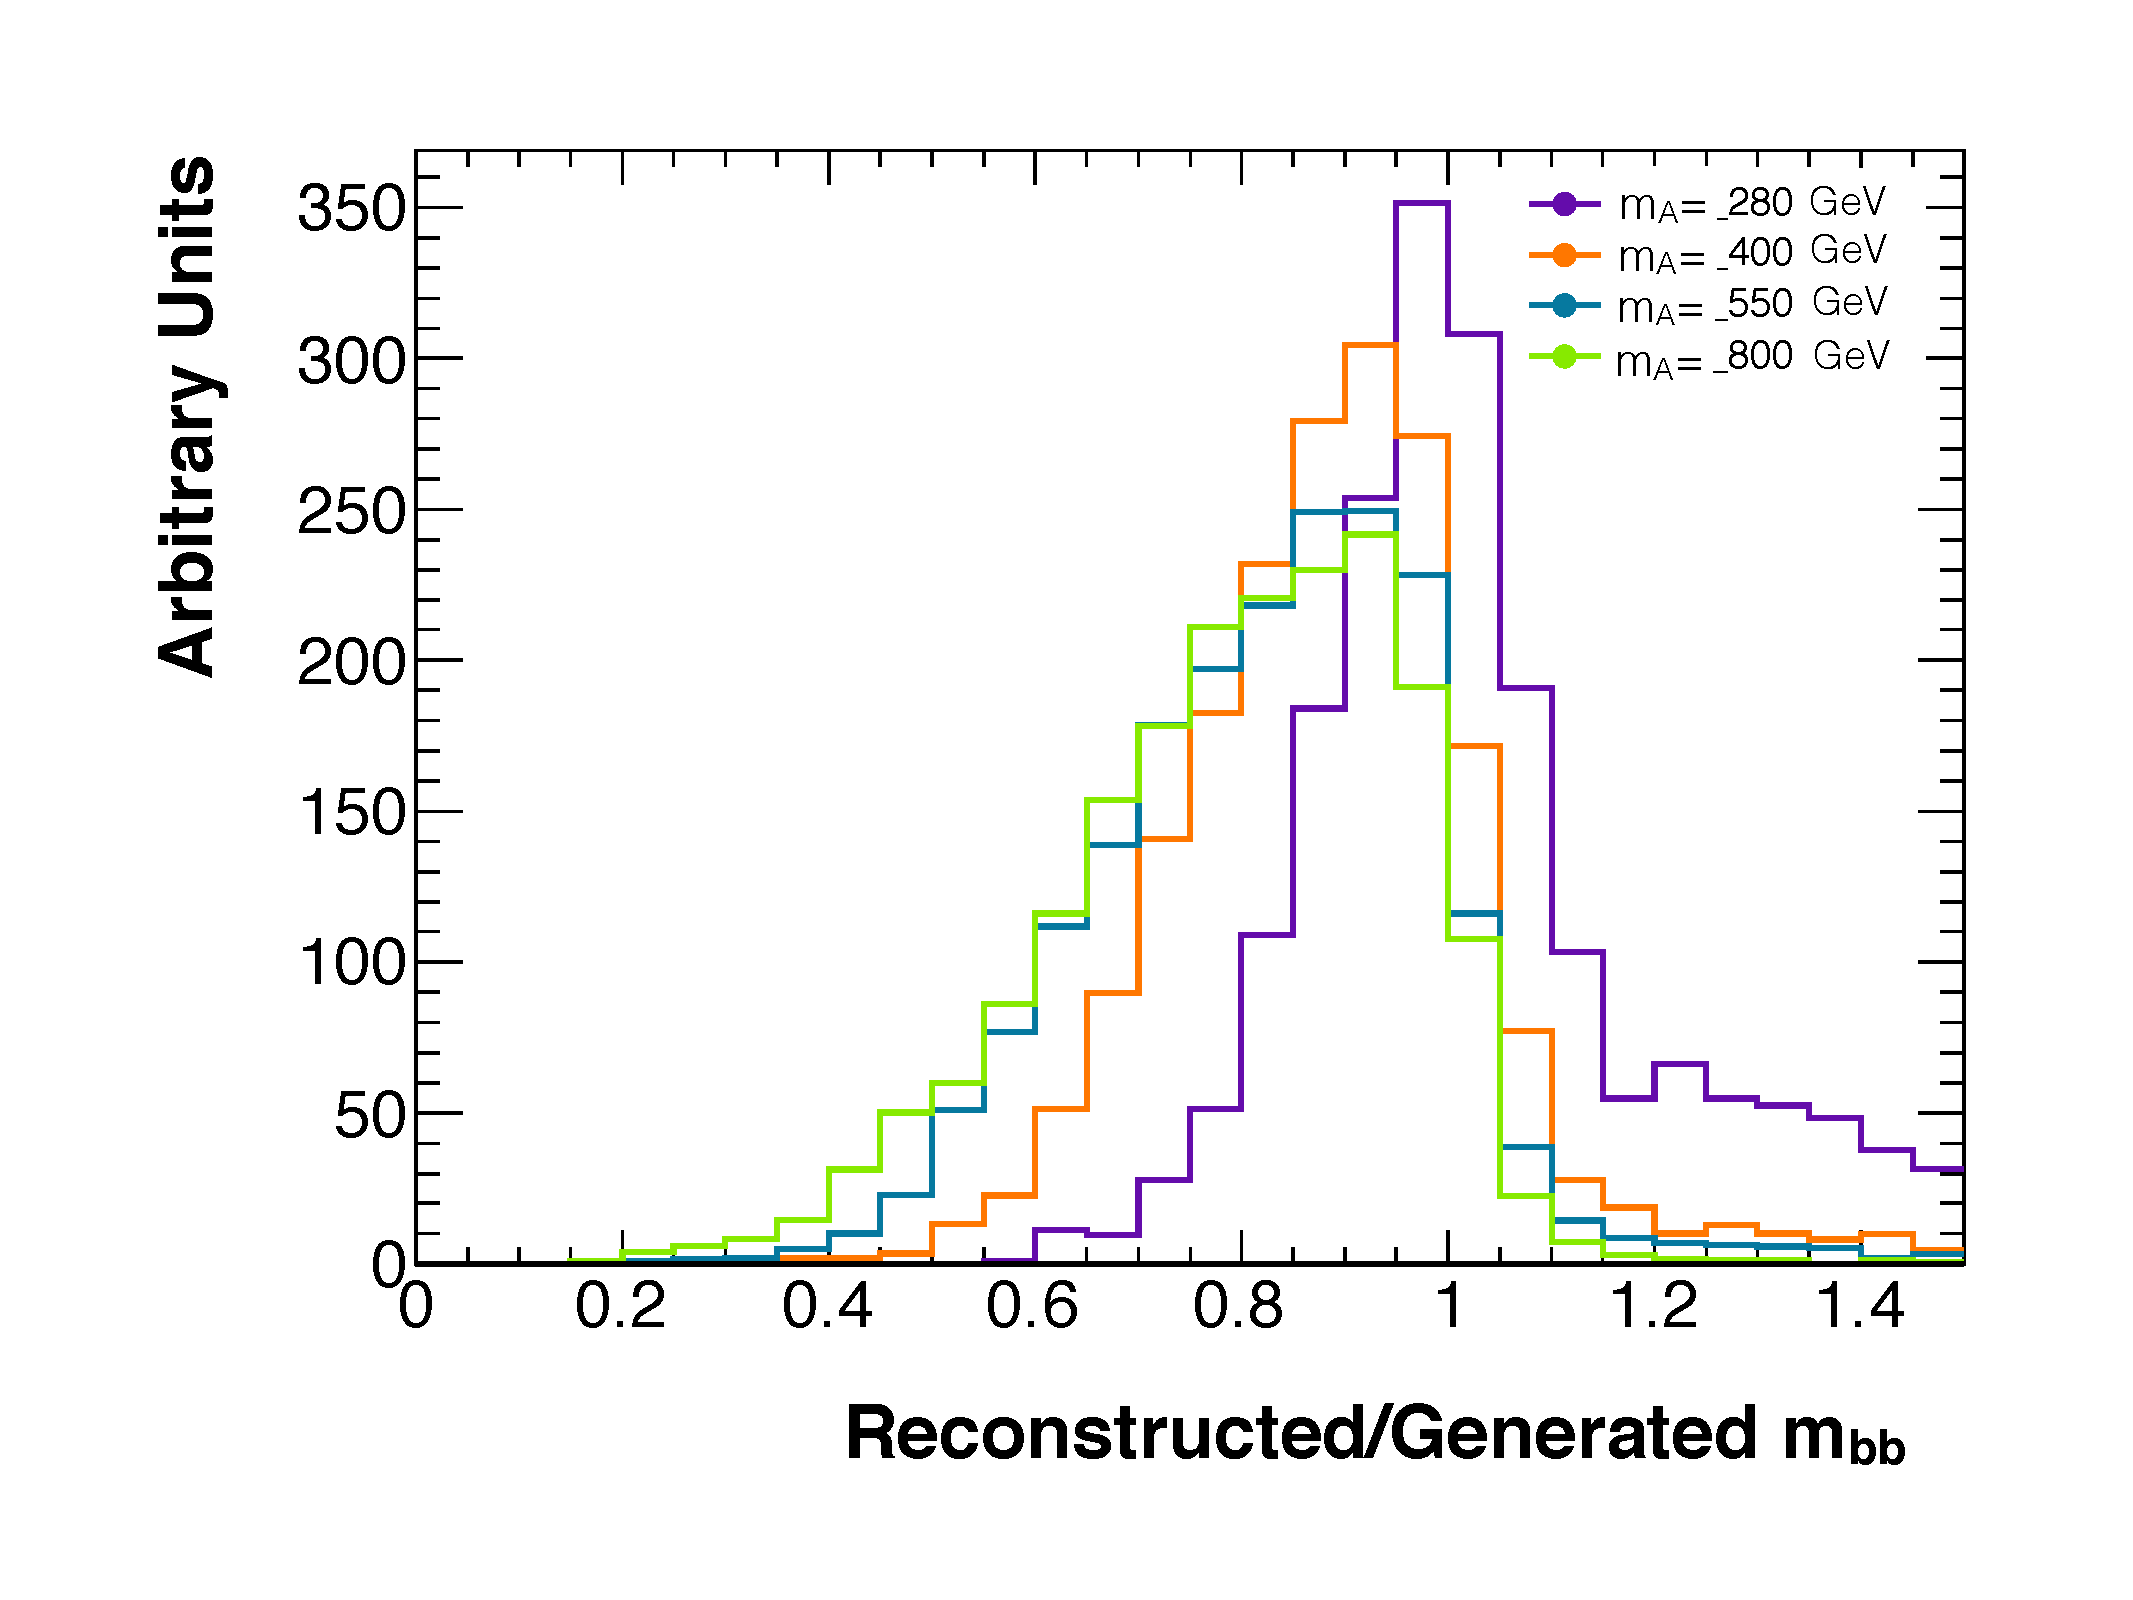
\includegraphics[width=0.78\linewidth]{SignalKin/mbb_normalized_signal.pdf}
  \label{fig:mbb_norm}
  \caption{The normalized $m_{bb}$ distributions for several signal mass points}
\end{figure}





\subsection{Jet Reconstruction Modifications}
As noted in Section~\ref{sec:jet_reco}, this analysis uses anti-$k_t$ jets with a distance parameter
of R=0.4.  It is possible that, for a signficant number of jets, some of the radiation associated
with the jet is falling outside of the jet radius and is therefore lost during clustering and
reconstruction.  A way to test this hypothesis is to reconstruct the signal events with R=0.6
jets, and see if the mass resolution improves. 

We find that the mass resolution does get marginally better (narrower distribution and higher mean
for the $m_{bb}$ distribution) for high-mass signal MC events, but only by a few percent.
Practical concerns prevent R=0.6 jets from being a serious consideration: first, the background
would also be pushed toward higher masses as QCD jets are reconstructed with larger radii;
second, pileup calibration and removal would be a significantly larger concern; and third,
the $b$-tagging calibrations are created only for R=0.4 jets so the $b$-tagging systematics
would be much more difficult to quantify.  


\subsection{Topology-Based Energy Recovery Algorithm}
 One hypothesis for the distribution of the FSR is that, for the high-\pt jets that result from the Higgs
 daughter b-quarks, they might radiate away partons that are hard enough to be clustered into their own
 jets (\pt$>$25 GeV) but end up nearby the leading jets in the detector (where nearby is defined as within
 dR$<$1.0). In other words, we look for a topology where there are one or more jets near one of the leading
2 jets, and in cases where such jets are found, we add them back in when reconstructing mbb.
 This is found to have little ect on the mass resolution. In practice, only about 20\% of events
 have the topology where additional jet(s) are found near the leading 2 jets, and the mass resolution
 looks virtually unchanged before and after adding this correction. This suggests a couple of possible
 conditions: either the FSR is too diffuse and/or low-energy to be clustered into jets, and/or it is farther
 than the dR $<$ 1.0 search zone allows for recovery. 
    
\begin{figure}[hbt]
  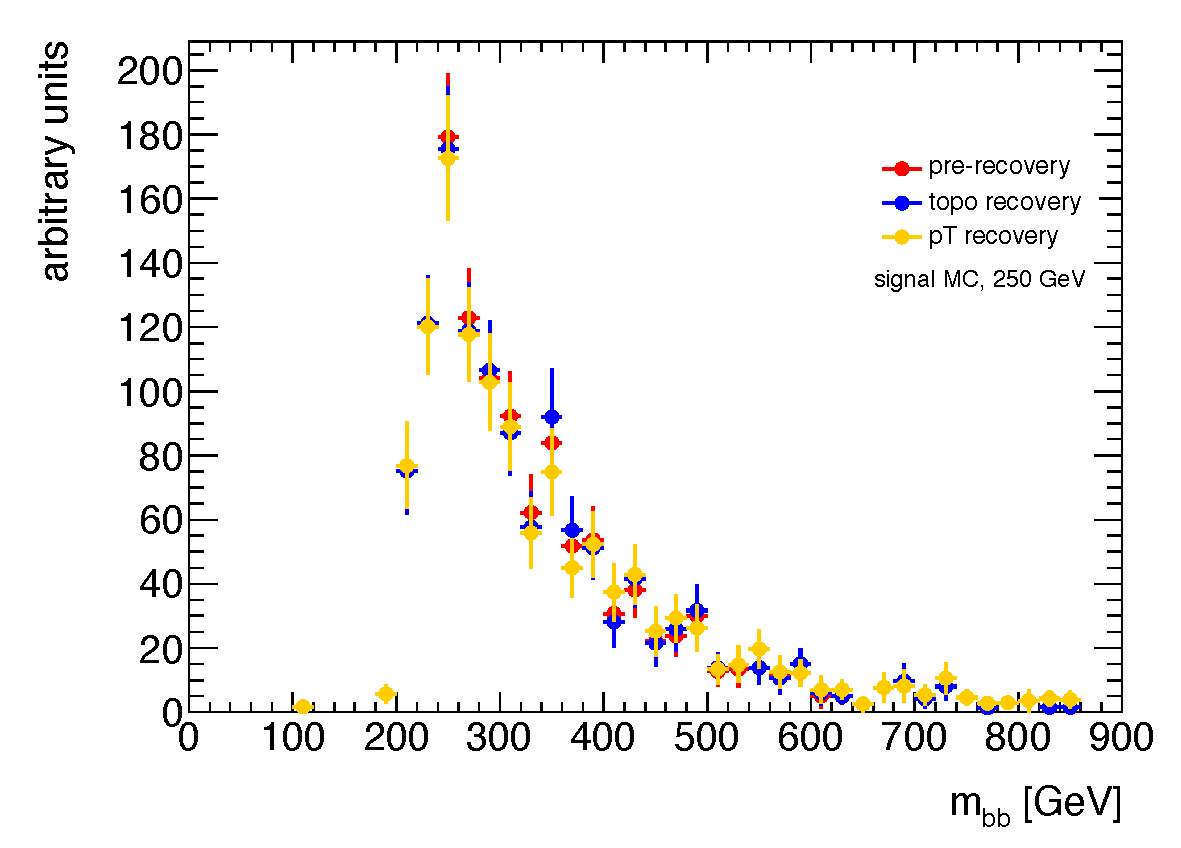
\includegraphics[width=0.45\linewidth]{SignalKin/fsr_recovery_bAbb_250.pdf}
  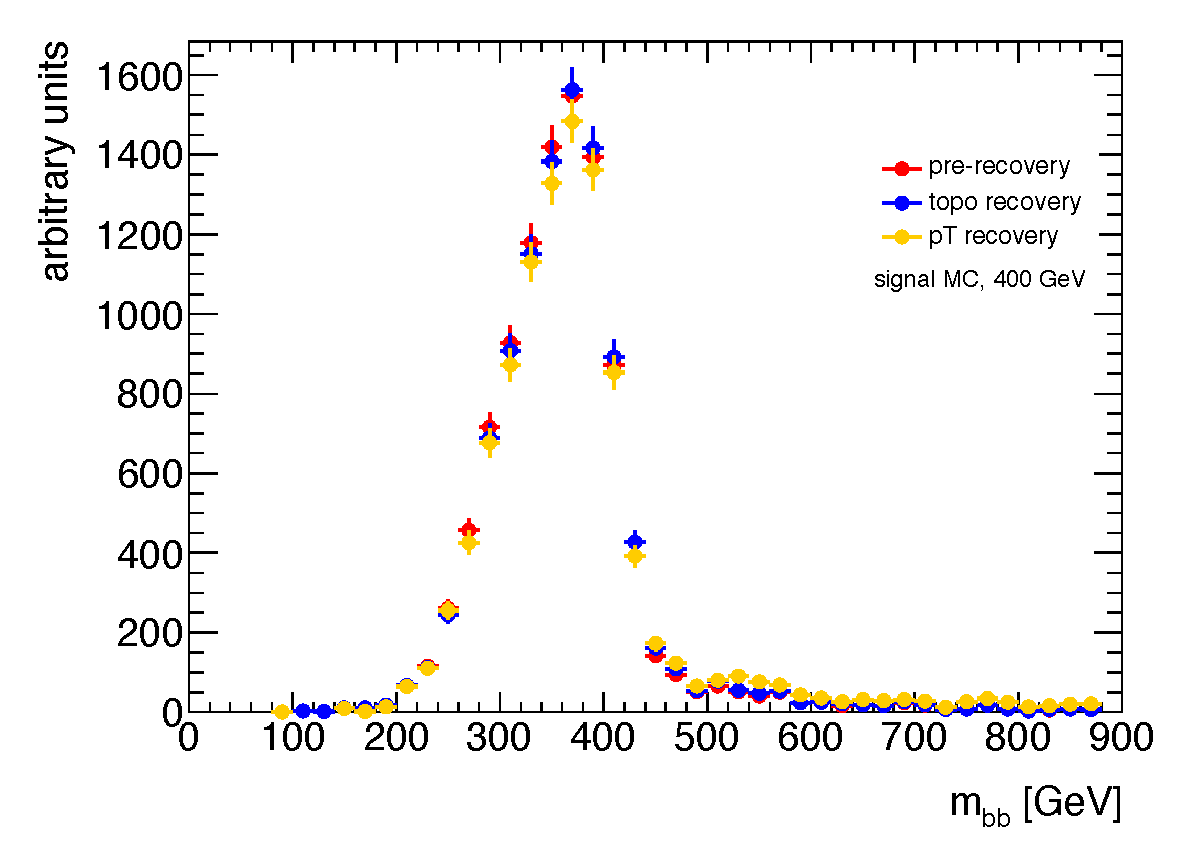
\includegraphics[width=0.45\linewidth]{SignalKin/fsr_recovery_bAbb_400.pdf}
\newline
  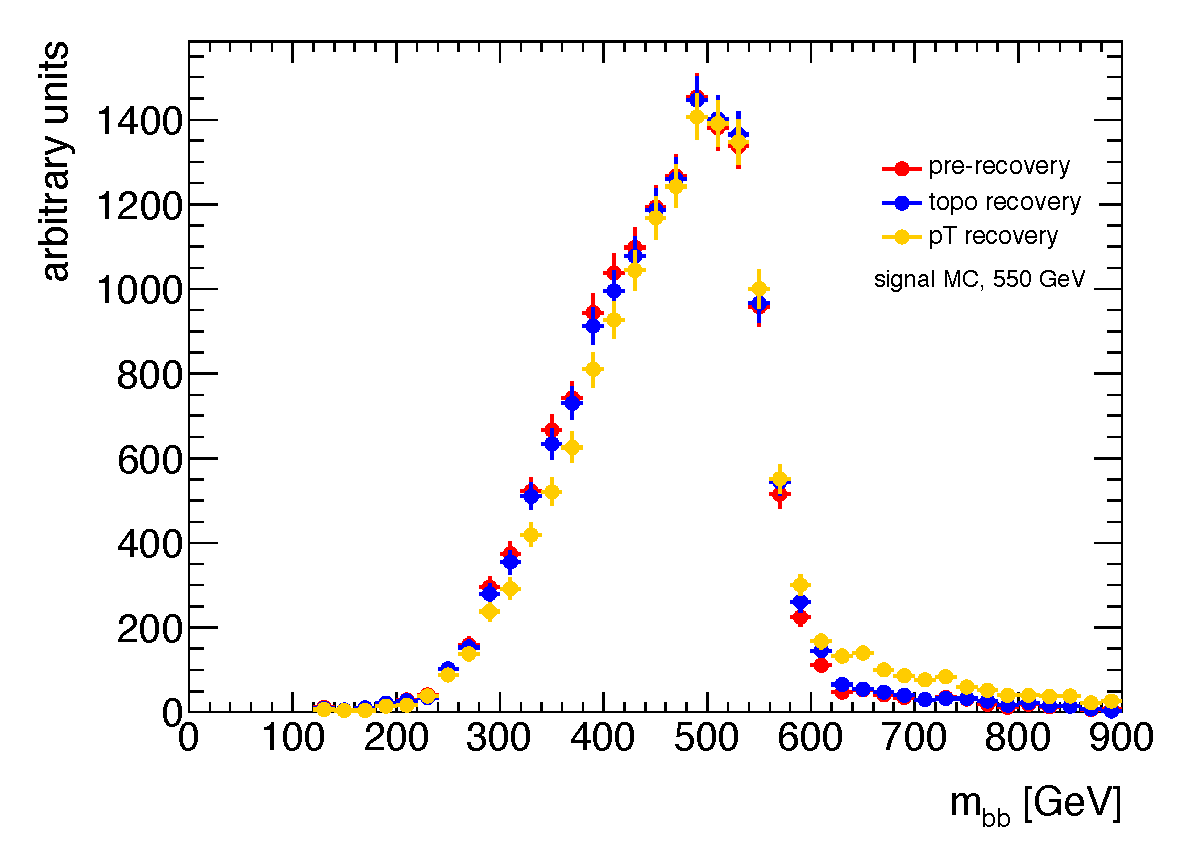
\includegraphics[width=0.45\linewidth]{SignalKin/fsr_recovery_bAbb_550.pdf}
  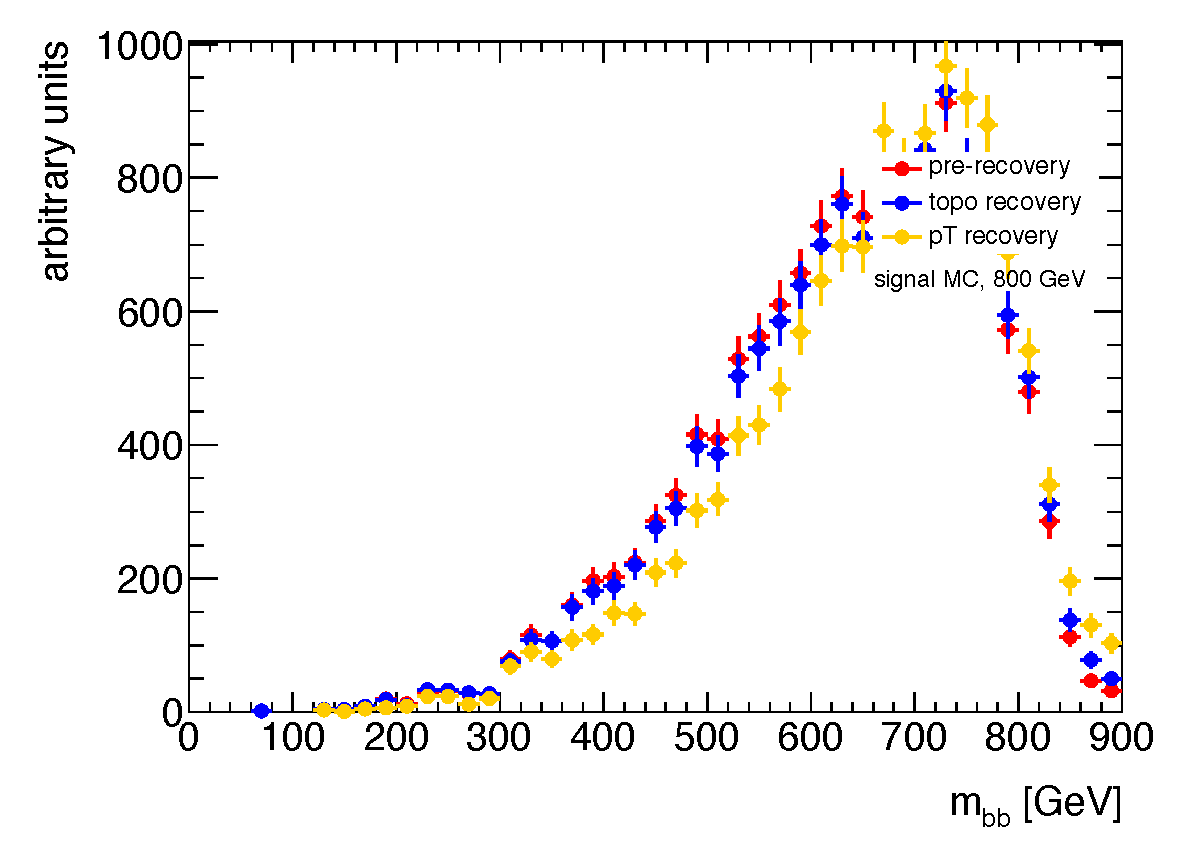
\includegraphics[width=0.45\linewidth]{SignalKin/fsr_recovery_bAbb_800.pdf}
  \label{fig:fsr_recovery}
  \caption{The $m_{bb}$ distributions out-of-the-box, and after attempting the $p_T$-based and topology-based FSR recovery algorithms, for several signal mass points.}
\end{figure}



\subsection{\pt-Based Energy Recovery Algorithm}
The \pt-based energy recovery algorithm is based on the idea that perhaps the FSR takes the form of one
 or two very high-energy radiated particles that can end up far away from the leading 2 jets but can be
 identified by their high pT . In practice, what this means is looking for events with a non-b-tagged jet that
 has \pt$>$80 GeV, and when one is found, adding this back in when reconstructing mbb.
 Unfortunately the ect on the mass resolution is negligible. A few events move out of the low-mass
 tail, and the high-mass tail gets a few more events as jets can be mistakenly added back in even when no
 FSR was lost.






\subsection{$n_{jets}$ Dependence}
\label{sec:n_jets_sig}

The signal mass resolution also displays a large dependence on $n_{jets}$, the 
number of jets over 25 GeV in the event.  If the event has significant FSR,
that radiation can end up clustered into extra jets in the event, and the 
mass resolution suffers at the same time.  In events where there are only 3 jets,
we can say rather confidently that two of the jets come from the Higgs decay
and the third is from the associated production; as long as we pick the jets
properly, the mass resolution should not show major effects of FSR.  That 
better resolution propagates through to allow the fit an easier time in distinguishing
signal from background, and generally gives better sensitivity than 
when the signal has poor mass resolution, all other things being equal.  
That motivates our decision in the fitting step of the analysis to treat
the 3-jet, 4-jet, and 5 or more jet events separately, and only combine at the
end when computing the net sensitivity.  More details on that procedure can 
be found in Section~\ref{subsec:fitmodel}.



\begin{figure}[hbt]
  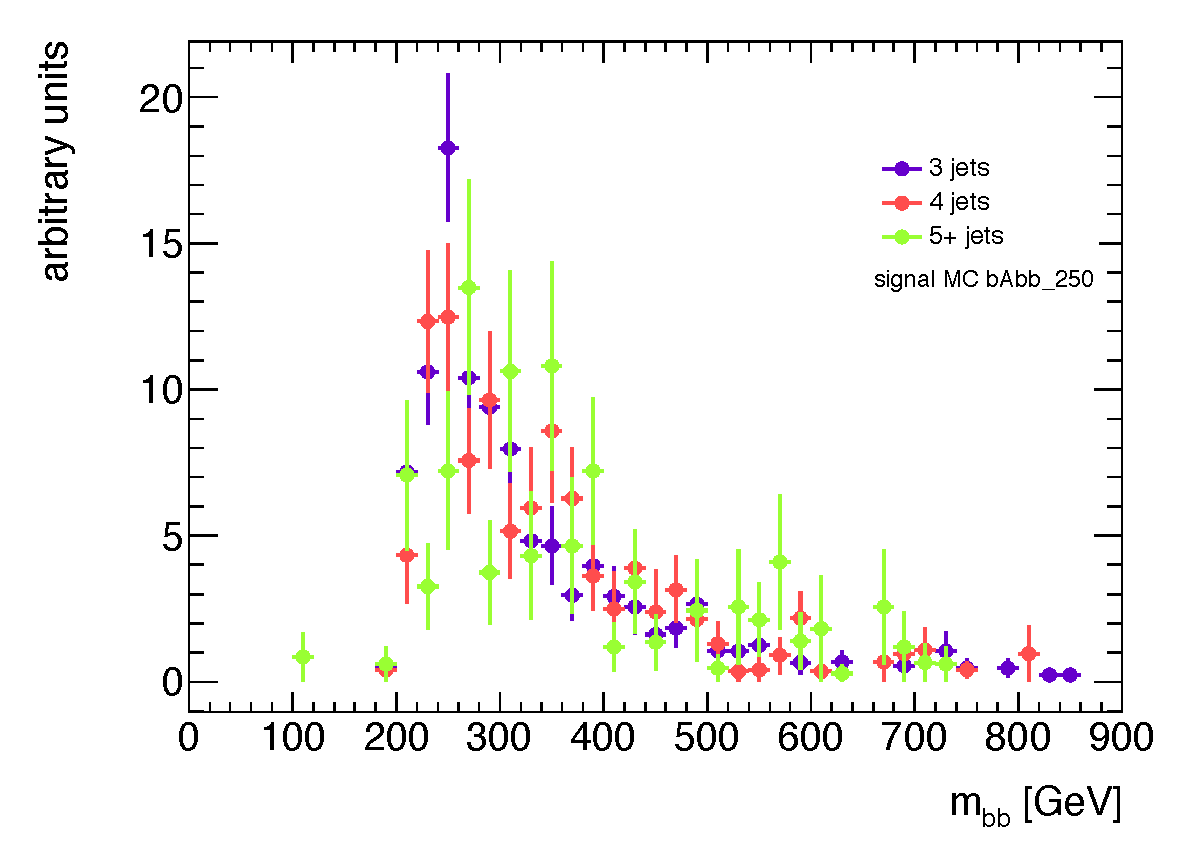
\includegraphics[width=0.45\linewidth]{SignalKin/mbb_njets_bAbb_250.pdf}
  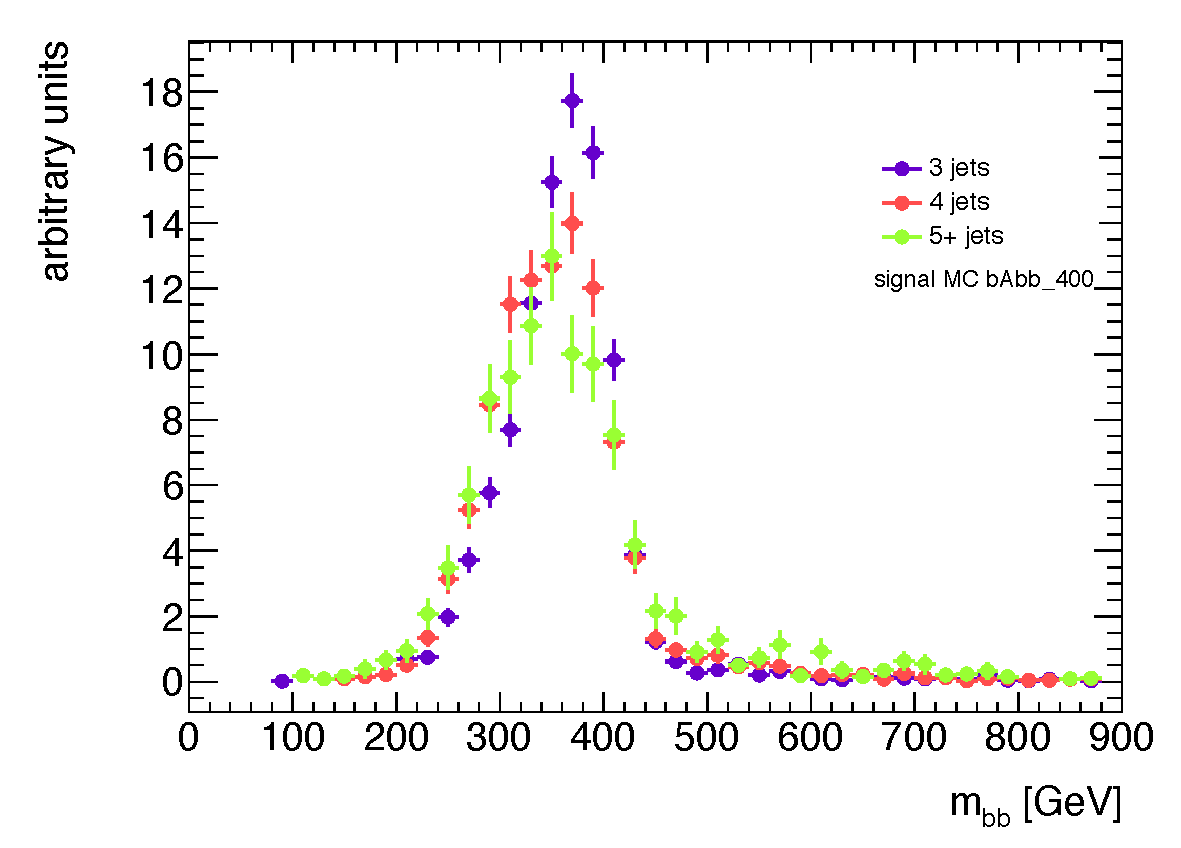
\includegraphics[width=0.45\linewidth]{SignalKin/mbb_njets_bAbb_400.pdf}
\newline
  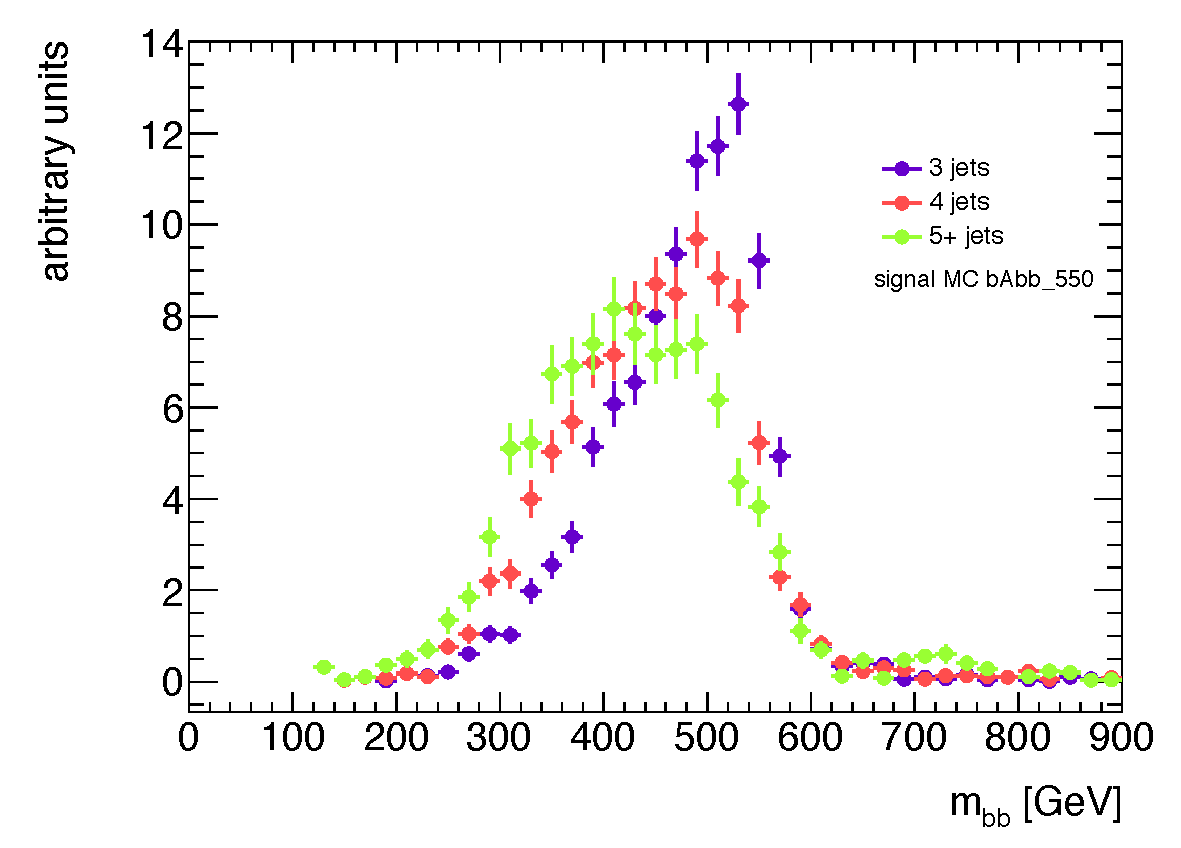
\includegraphics[width=0.45\linewidth]{SignalKin/mbb_njets_bAbb_550.pdf}
  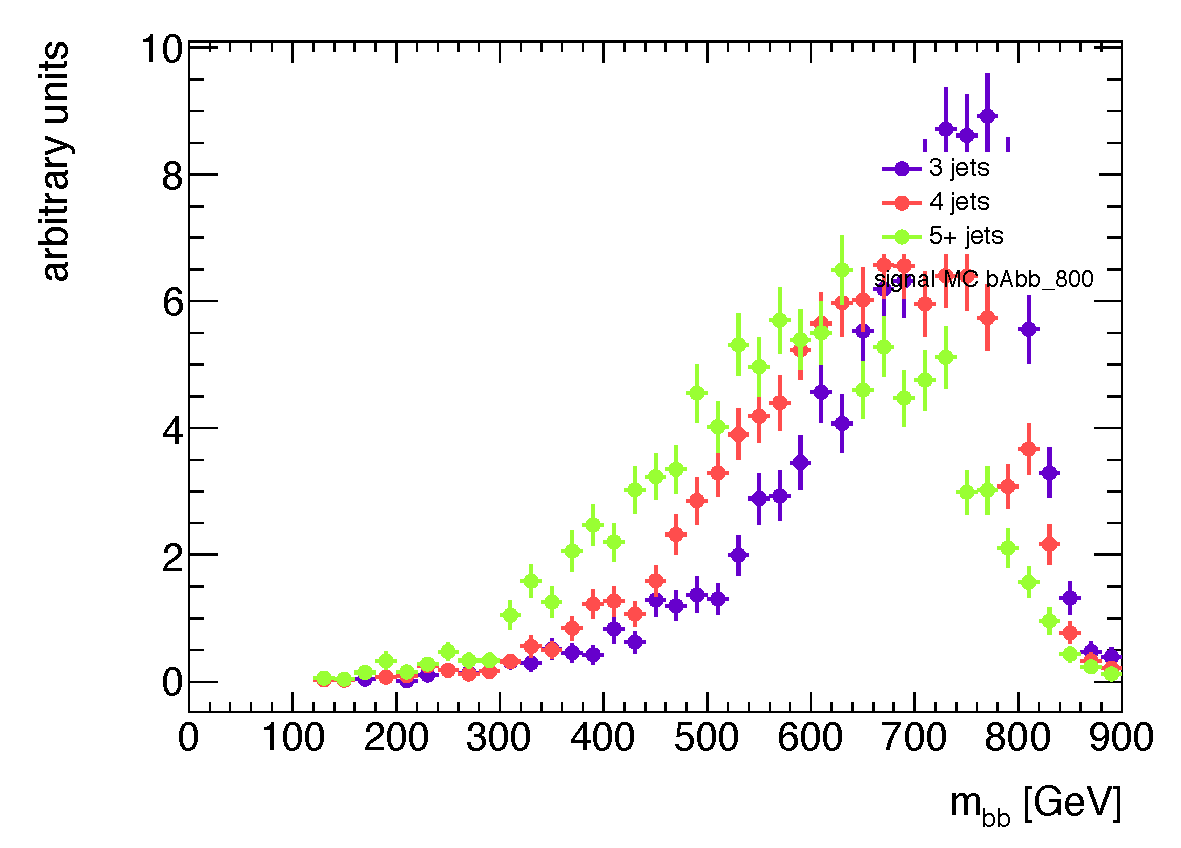
\includegraphics[width=0.45\linewidth]{SignalKin/mbb_njets_bAbb_800.pdf}
  \label{fig:mbb_njets_signal}
  \caption{The $m_{bb}$ distributions at a few representative mass points in signal MC, as a function of the number of jets in the event.  
    The 5+ jets bin contains all events with 5 jets or more.}
\end{figure}


\section{Eigenvector Rotation}
\label{sec:rotation}
%\begin{itemize}
%    \item for high-mass points, we have trouble when FSR is bad (but it isn't always bad)
%    \item FSR is worst when jets are low-pT--suggests a cut or categorization based
%    on pT of the jets
%    \item However, simple cut can sculpt background b/c of correlations btwn pT1, pT2, mbb,
%    and it also reduces background to rates too low to model well
%    \item use signal MC to identify eigenvectors based on pT1, pT2 and mbb, transform
%    into this basis 
%    \item Place cuts on pT1' and pt2'
%    \item Use $mbb'$ as the discriminating variable, proceed to fit with exponential
%    \item Impact on final sensitivity in the results section
%\end{itemize}

Once the events have been categorized based on $b$-tag status and the number of jets in the
events, but before doing the final fit, we apply a change of variables based on the jet
$p_T$ values and $m_{bb}$ in each event and a kinematic cut.  Together these analysis 
steps effectively allow for a discriminating variable, which we call $m_{bb}'$, that
separates signal and background better than ordinary $m_{bb}$.  Once these steps have
been applied, the result is an analysis that is 15-50\% more sensitive
than if no transformation were applied.  This section will 
outline this procedure and its rationale.  

The motivation for this strategy has its origins in trying to control the effect of
FSR on the analysis sensitivity.  At high $m_A$, the jets from the Higgs (and also 
the associated $b$-quark) have large $p_T$, which they then tend to radiate away 
as FSR.  This causes the $m_{bb}$ peak to smear out and be more difficult to 
distinguish from background than in the lower-$m_A$ cases.  However, since FSR
occurs stochastically on an event-by-event basis, a subset of the signal events
will have little or no FSR and will reconstruct to $m_A$--if these events 
can be isolated from the others, they offer a chance to improve the sensitivity
via the improved mass resolution and signal-to-background ratio. 

A simple strategy might be to apply a cut to the $p_T$ of the leading and/or 
second jet in the event, and only accept events where the $p_T$ is above some
threshold optimized by comparing signal MC to \textit{bbanti} data.  
That would isolate events with poor mass resolution (i.e. lots of FSR) from
those with little FSR and better reconstruction properties.  However, since
there is a correlation between $p_T^1$, $p_T^2$ and $m_{bb}$, a cut like
this ends up sculpting the background as well.  In addition, the $p_T^1$ and
$p_T^2$ cut thresholds that looked best on signal MC are ``too good'' on 
background-dominated \textit{bbanti} events and there is no background
above a certain $m_{bb}$ value.  That makes modeling the background extremely 
difficult, and any fit difficult to validate.  

The rotation is performed as follows:
\begin{itemize}
    \item For $m_{bb}$, $p_T^1$ and $p_T^2$ calculate the center of gravity
    of all signal MC simulation events, and subtract it from each event
    \item For each event, fill a 3$\times$3 tensor with the following components
    \begin{equation}
        \begin{bmatrix}
        m_{bb}m_{bb} & m_{bb}p_T^1 & m_{bb}p_T^2 \\
                     & p_T^1 p_T^1 & p_T^1 p_T^2 \\
                     &             & p_T^2 p_T^2 \\ 
        \end{bmatrix}
    \end{equation}
    (the matrix is symmetric, so we write only the elements above the diagonal for
    brevity and clarity)
    \item Sum these tensor matrices for all signal events in a given tag/jet category
    (the resulting tensor will also be 3$\times$3)
    \item Find the leading eigenvector\footnote{where the leading eigenvector is the
    eigenvector associated with the largest eigenvalue} of the tensor matrix
    \item Define the $m_{bb}^{'}$ variable as follows:
    \begin{equation}
        m_{bb}^{'} = [m_{bb}\ p_T^1\ p_T^2] \cdot [e_1\ e_2\ e_3]
    \end{equation}
    where the latter vector is the leading eigenvector of the tensor matrix
\end{itemize}

After this rotation, $m_{bb}^{'}$ is an admixture of $m_{bb}$, $p_T^1$, and 
$p_T^2$.  The exact contribution from each of these variables changes on a mass-point-by-mass-point
basis, as the correlations between them change.  At lower masses, $m_{bb}$ provides
most of the basis for $m_{bb}^{'}$, with 76\% of the $m_{bb}^{'}$ coming from 
$m_{bb}$.  At higher masses, where FSR is more of an issue, the correlations between 
$m_{bb}$ and the leading jets' $p_T$s are more important and for $m_A$=800 GeV,
over half of $m_{bb}^{'}$ (55\%) comes from $p_T^1$ and $p_T^2$.  The full set 
of $m_{bb}^{'}$ components can be found in Table~\ref{tab:eigenvector_elements}.


%Adding a change of basis before the $p_T$ cuts turns out to offer the advantage
%of better signal/background separation without the cost of making the background
%difficult to model.  The basis change is a rotation away from the $p_T^1$, 
%$p_T^2$, $m_{bb}$ basis into what we call the $p_T^{1'}$, $p_T^{2'}$, $m_{bb}^{'}$
%basis, where $p_T^{1'}$, $p_T^{2'}$, $m_{bb}^{'}$ are the eigenvectors of 
%a matrix built out of $p_T^1$, $p_T^2$, and $m_{bb}$.  The leading eigenvector 
%\footnote{the leading eigenvector is defined as the eigenvector with the largest
%associated eigenvalue}, which we call $m_{bb}^{'}$, is an admixture of 
%$p_T^1$, $p_T^2$, and $m_{bb}$, the exact blend of which varies by signal mass
%point.  The relative contributions of $p_T^1$, $p_T^2$, and $m_{bb}$ to the $m_{bb}^{'}$
%leading eigenvector can be seen in Table~\ref{tab:eigenvector_elements}.


\begin{table}
    \center
    \caption{The major axis eigenvector elements, and their squares.  The
    transformation into the eigenbasis makes use of the raw elements, but the
    squares of the elements sum to 1.0 and can provide some physical intuition
    for the relative contributions of $p_T^1$, $p_T^2$ and $m_{bb}$. \label{tab:eigenvector_elements}}
    \begin{tabular}{ c c c c c c c } \hline \hline
        $m_A$ & $m_{bb}$ & $p_T^1$ & $p_T^2$ & $m_{bb}^2$ & $(p_T^{1})^2$ & $(p_T^2)^2$ \\ \hline
        450 & 0.87 & 0.35 & 0.35 & 0.76 & 0.12 & 0.12 \\
        500 & 0.84 & 0.38 & 0.39 & 0.71 & 0.14 & 0.15 \\
        550 & 0.80 & 0.40 & 0.46 & 0.64 & 0.16 & 0.21 \\
        600 & 0.78 & 0.41 & 0.47 & 0.61 & 0.17 & 0.22 \\
        650 & 0.72 & 0.46 & 0.52 & 0.52 & 0.21 & 0.27 \\
        700 & 0.71 & 0.47 & 0.54 & 0.50 & 0.22 & 0.29 \\
        800 & 0.67 & 0.50 & 0.55 & 0.45 & 0.25 & 0.30 \\ 
        \hline
    \end{tabular}
\end{table} 

The effect of this transformation on 450 and 800 GeV signal and background-dominated
data can be seen in Figure ~\ref{fig:transformed_vars}.  These figures show
the difference in the $m_{bb}$ distributions %and $p_T$ distributions 
before and after the transformation,
with the mass distribution being pushed to lower values
in the background distribution while the signal mass maintains a similar shape.  
This background reshaping affects the signal to background ratio in the 
neighborhood of the signal peak; before the rotation,
significant background remaining in the neighborhood of the signal peak, 
but after the rotation the signal is virtually
unchanged while the background has been shifted lower.  

\begin{figure}[hbt]
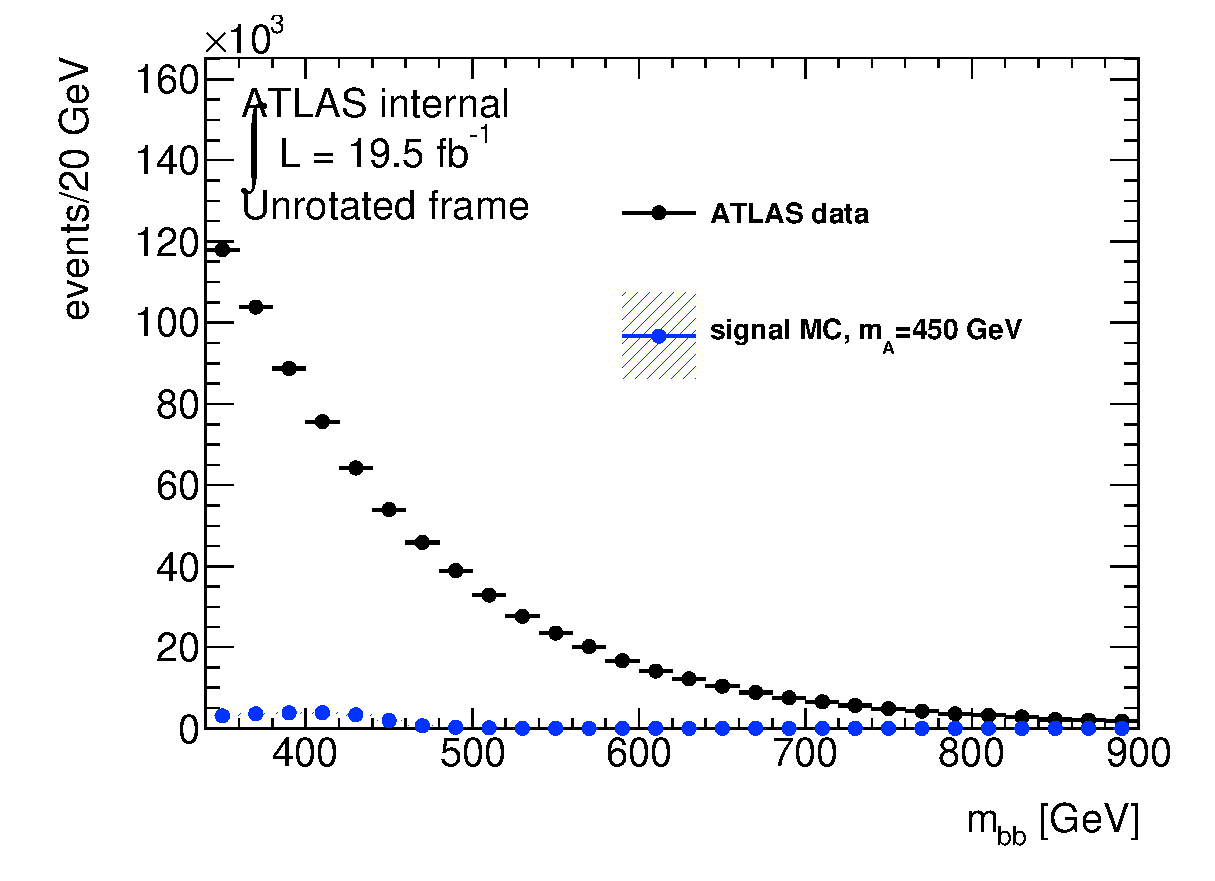
\includegraphics[width=0.45\linewidth]{SignalKin/h_mass_bAbb_450_unrotated.eps}
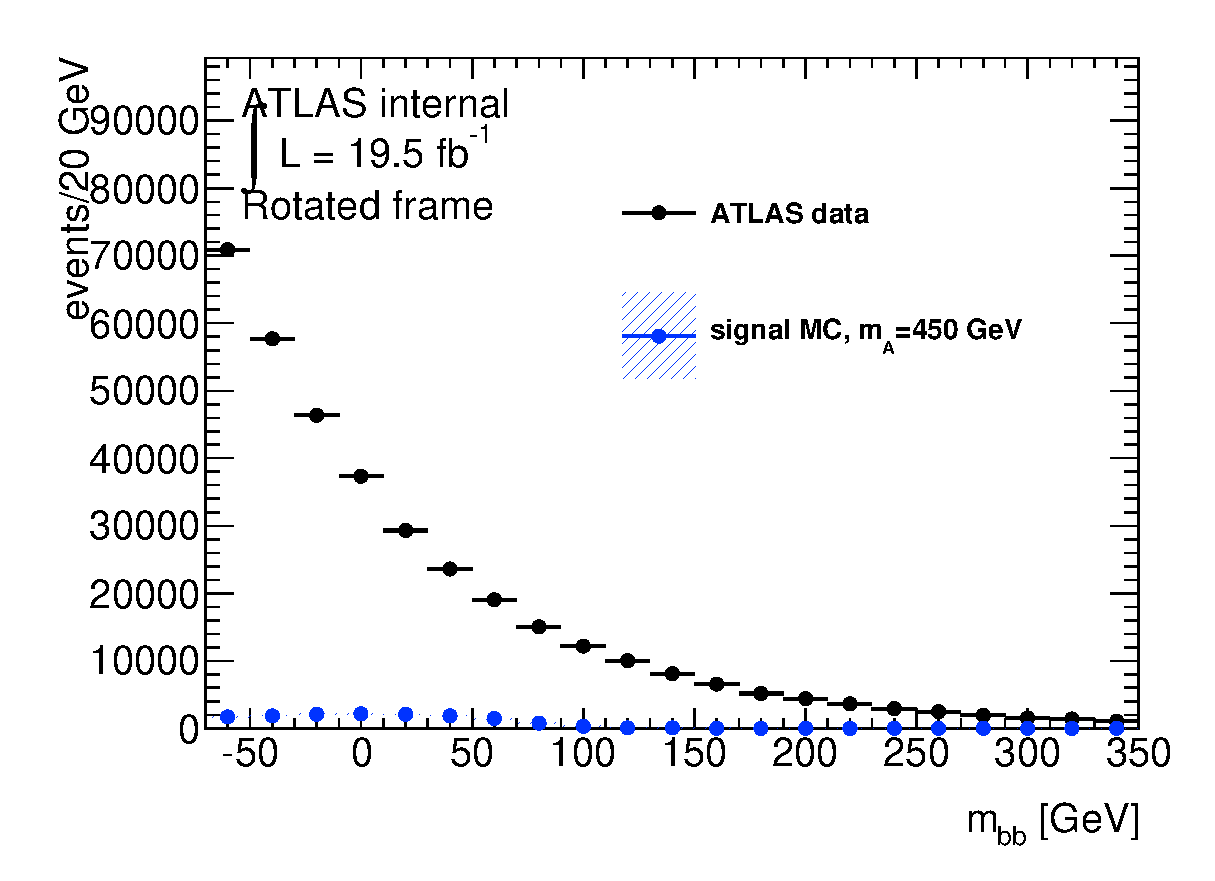
\includegraphics[width=0.45\linewidth]{SignalKin/h_mass_bAbb_450_rotated.eps} \\
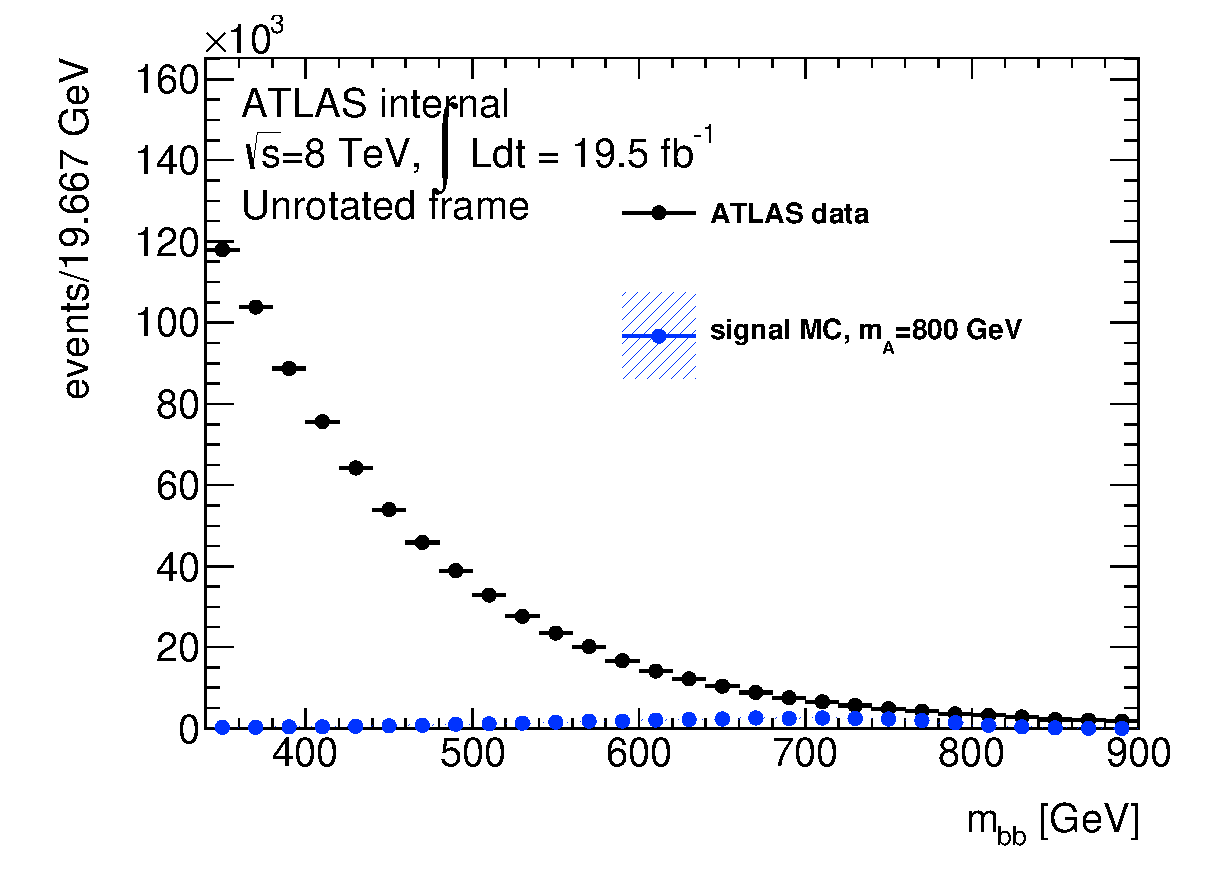
\includegraphics[width=0.45\linewidth]{SignalKin/h_mass_bAbb_800_unrotated.eps}
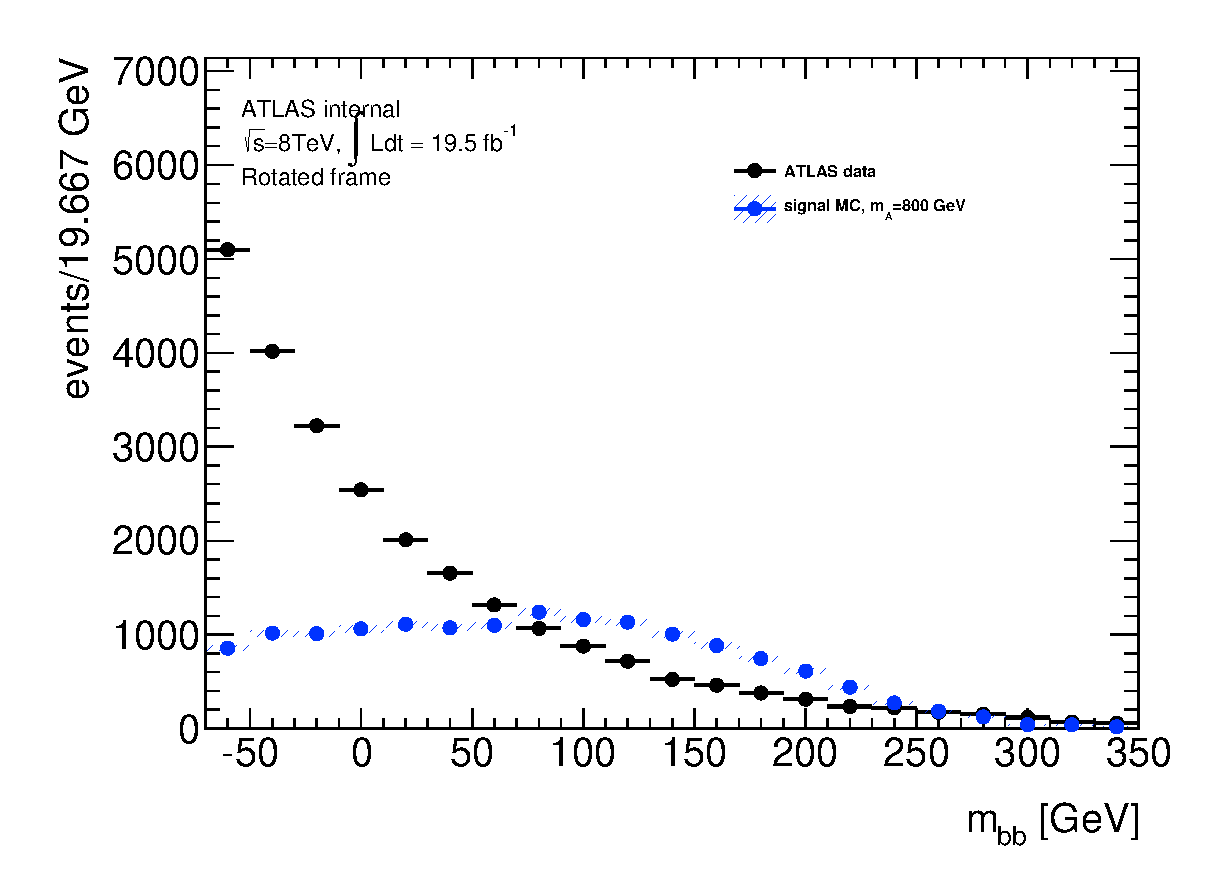
\includegraphics[width=0.45\linewidth]{SignalKin/h_mass_bAbb_800_rotated.eps} \\
\caption{ Comparisons of the signal and background $m_{bb}$ distributions
    before and after the rotation.  The left two plots show 450 GeV and 800 GeV
    Higgs mass points before the rotation. The signal is extremely small compared to the background, whereas the 
    same distributions (including the same signal normalization) after the rotation
    are on the right, for the same two mass points.  The rotation pushes the
    background events to lower values of $m_{bb}^{'}$ than the signal, yielding
    better signal/background separation, especially for higher mass Higgs candidates.
     \label{fig:transformed_vars}}
\end{figure}


While the $m_{bb}^{'}$ variable is derived using the leading eigenvector of the
tensor matrix, the second and third eigenvectors can also be used in an analagous
way and we refer to the resulting transformed variables as $p_T^{1'}$ and $p_{T}^{2'}$.


There is one more step that optimizes the signal to background
discrimination further, which is placing cuts on $p_T^{1'}$ and $p_T^{2'}$.
If we require that $p_T^{1'}>-10$ GeV, and $p_T^{2'}>-50$ GeV, it 
excludes a region of $m_{bb}^{'}$ phase space where the modeling is difficult
and little sensitivity is gained.  








\subsubsection{Binned Fit to Signal}

The signal shape is fit using an RhhBinnedPdf in RooFit, a form of parameterized
histogram where the parameterization helps the fit converge more reliably and allows
a single parameter to capture the integral (i.e. signal yield) of the distribution.
Once the full analysis cut chain has been applied, including the rotation, the 
signal $m_{bb}$ distributions are fit in signal MC and then the shapes are fixed.
The mass range for the signal fits (and also the background fits) is -50 GeV $< m_{bb}^{'}<$ 350 GeV,
and the bins are 40 GeV wide in a compromise between trying to capture as much
shape information as possible while also dealing with limited signal MC statistics.

The choice of a parameterized histogram was taken after it was found that 
the signal distribution is a difficult one to fit to a function, since the shape can vary
widely by jet bin and $b$-tag category.  Attempts to fit the distributions with e.g. a 
Cruijff function (a bifurcated Gaussian function with non-Gaussian tails) would work
well for some categories and signal mass points, but fail to give good shape descriptions
for other categories and signal mass points.  By fitting to a histogram, we are able
to fit trickier shapes than could be reliably fit with a function, and the fits are
more stable under the addition of perturbations from systematic errors.


%http://www.slac.stanford.edu/econf/C0303241/proc/pres/502.PDF
%The signal $m_{bb}$ shape is fit with a Cruijff PDF.  The Cruijff function is a 
%bifurcated Gaussian (different widths for left and right sides of the distribution) with non-Gaussian tails: 

%\begin{equation}
%f(x) = exp((x-m_{bb})^2 / (2\sigma^2_{L,R} + \alpha_{L,R}(x-m)^2))
%\end{equation}

%The signal MC distributions and fit results can be seen in Figures


\begin{figure}[phtb!]
  \begin{center}
  \begin{subfigure}[$m_{A}=400$ GeV]{0.4\textwidth}\includegraphics[width=\textwidth]{SignalKin/fitMC_bAbb_400_bbb_3jets_formatted.eps}\end{subfigure}
  \begin{subfigure}[$m_{A}=450$ GeV]{0.4\textwidth}\includegraphics[width=\textwidth]{SignalKin/fitMC_bAbb_450_bbb_3jets_formatted.eps}\end{subfigure}
  \begin{subfigure}[$m_{A}=500$ GeV]{0.4\textwidth}\includegraphics[width=\textwidth]{SignalKin/fitMC_bAbb_500_bbb_3jets_formatted.eps}\end{subfigure}
  \begin{subfigure}[$m_{A}=550$ GeV]{0.4\textwidth}\includegraphics[width=\textwidth]{SignalKin/fitMC_bAbb_550_bbb_3jets_formatted.eps}\end{subfigure}
  \begin{subfigure}[$m_{A}=600$ GeV]{0.4\textwidth}\includegraphics[width=\textwidth]{SignalKin/fitMC_bAbb_600_bbb_3jets_formatted.eps}\end{subfigure}
  \begin{subfigure}[$m_{A}=650$ GeV]{0.4\textwidth}\includegraphics[width=\textwidth]{SignalKin/fitMC_bAbb_650_bbb_3jets_formatted.eps}\end{subfigure}
  \begin{subfigure}[$m_{A}=700$ GeV]{0.4\textwidth}\includegraphics[width=\textwidth]{SignalKin/fitMC_bAbb_700_bbb_3jets_formatted.eps}\end{subfigure}
  \begin{subfigure}[$m_{A}=800$ GeV]{0.4\textwidth}\includegraphics[width=\textwidth]{SignalKin/fitMC_bAbb_800_bbb_3jets_formatted.eps}\end{subfigure}
  \caption{Signal MC distributions and RhhBinnedPdf PDFs for $m_{bb}$ in the {\it bbb} category, for events with 3 jets, for different $H/A$ masses after the rotation has been applied.\label{fig:signalPDFs_3j_bbb}} 
    \end{center}
\end{figure}


\begin{figure}[phtb!]
  \begin{center}
  \begin{subfigure}[$m_{A}=400$ GeV]{0.4\textwidth}\includegraphics[width=\textwidth]{SignalKin/fitMC_bAbb_400_bbb_4jets_formatted.eps}\end{subfigure}
  \begin{subfigure}[$m_{A}=450$ GeV]{0.4\textwidth}\includegraphics[width=\textwidth]{SignalKin/fitMC_bAbb_450_bbb_4jets_formatted.eps}\end{subfigure}
  \begin{subfigure}[$m_{A}=500$ GeV]{0.4\textwidth}\includegraphics[width=\textwidth]{SignalKin/fitMC_bAbb_500_bbb_4jets_formatted.eps}\end{subfigure}
  \begin{subfigure}[$m_{A}=550$ GeV]{0.4\textwidth}\includegraphics[width=\textwidth]{SignalKin/fitMC_bAbb_550_bbb_4jets_formatted.eps}\end{subfigure}
  \begin{subfigure}[$m_{A}=600$ GeV]{0.4\textwidth}\includegraphics[width=\textwidth]{SignalKin/fitMC_bAbb_600_bbb_4jets_formatted.eps}\end{subfigure}
  \begin{subfigure}[$m_{A}=650$ GeV]{0.4\textwidth}\includegraphics[width=\textwidth]{SignalKin/fitMC_bAbb_650_bbb_4jets_formatted.eps}\end{subfigure}
  \begin{subfigure}[$m_{A}=700$ GeV]{0.4\textwidth}\includegraphics[width=\textwidth]{SignalKin/fitMC_bAbb_700_bbb_4jets_formatted.eps}\end{subfigure}
  \begin{subfigure}[$m_{A}=800$ GeV]{0.4\textwidth}\includegraphics[width=\textwidth]{SignalKin/fitMC_bAbb_800_bbb_4jets_formatted.eps}\end{subfigure}
  \caption{Signal MC distributions and RhhBinnedPdf PDFs for $m_{bb}$ in the {\it bbb} category, for events with 4 jets, for different $H/A$ masses after the rotation has been applied.\label{fig:signalPDFs_4j_bbb}} 
    \end{center}
\end{figure}


\begin{figure}[phtb!]
  \begin{center}
  \begin{subfigure}[$m_{A}=400$ GeV]{0.4\textwidth}\includegraphics[width=\textwidth]{SignalKin/fitMC_bAbb_400_bbb_5jets_formatted.eps}\end{subfigure}
  \begin{subfigure}[$m_{A}=450$ GeV]{0.4\textwidth}\includegraphics[width=\textwidth]{SignalKin/fitMC_bAbb_450_bbb_5jets_formatted.eps}\end{subfigure}
  \begin{subfigure}[$m_{A}=500$ GeV]{0.4\textwidth}\includegraphics[width=\textwidth]{SignalKin/fitMC_bAbb_500_bbb_5jets_formatted.eps}\end{subfigure}
  \begin{subfigure}[$m_{A}=550$ GeV]{0.4\textwidth}\includegraphics[width=\textwidth]{SignalKin/fitMC_bAbb_550_bbb_5jets_formatted.eps}\end{subfigure}
  \begin{subfigure}[$m_{A}=600$ GeV]{0.4\textwidth}\includegraphics[width=\textwidth]{SignalKin/fitMC_bAbb_600_bbb_5jets_formatted.eps}\end{subfigure}
  \begin{subfigure}[$m_{A}=650$ GeV]{0.4\textwidth}\includegraphics[width=\textwidth]{SignalKin/fitMC_bAbb_650_bbb_5jets_formatted.eps}\end{subfigure}
  \begin{subfigure}[$m_{A}=700$ GeV]{0.4\textwidth}\includegraphics[width=\textwidth]{SignalKin/fitMC_bAbb_700_bbb_5jets_formatted.eps}\end{subfigure}
  \begin{subfigure}[$m_{A}=800$ GeV]{0.4\textwidth}\includegraphics[width=\textwidth]{SignalKin/fitMC_bAbb_800_bbb_5jets_formatted.eps}\end{subfigure}
  \caption{Signal MC distributions and RhhBinnedPdf PDFs for $m_{bb}$ in the {\it bbb} category, for events with 5 jets, for different $H/A$ masses after the rotation has been applied.\label{fig:signalPDFs_4j_bbb}} 
    \end{center}
\end{figure}



\begin{figure}[phtb!]
  \begin{center}
  \begin{subfigure}[$m_{A}=400$ GeV]{0.4\textwidth}\includegraphics[width=\textwidth]{SignalKin/fitMC_bAbb_400_bbloose_3jets_formatted.eps}\end{subfigure}
  \begin{subfigure}[$m_{A}=450$ GeV]{0.4\textwidth}\includegraphics[width=\textwidth]{SignalKin/fitMC_bAbb_450_bbloose_3jets_formatted.eps}\end{subfigure}
  \begin{subfigure}[$m_{A}=500$ GeV]{0.4\textwidth}\includegraphics[width=\textwidth]{SignalKin/fitMC_bAbb_500_bbloose_3jets_formatted.eps}\end{subfigure}
  \begin{subfigure}[$m_{A}=550$ GeV]{0.4\textwidth}\includegraphics[width=\textwidth]{SignalKin/fitMC_bAbb_550_bbloose_3jets_formatted.eps}\end{subfigure}
  \begin{subfigure}[$m_{A}=600$ GeV]{0.4\textwidth}\includegraphics[width=\textwidth]{SignalKin/fitMC_bAbb_600_bbloose_3jets_formatted.eps}\end{subfigure}
  \begin{subfigure}[$m_{A}=650$ GeV]{0.4\textwidth}\includegraphics[width=\textwidth]{SignalKin/fitMC_bAbb_650_bbloose_3jets_formatted.eps}\end{subfigure}
  \begin{subfigure}[$m_{A}=700$ GeV]{0.4\textwidth}\includegraphics[width=\textwidth]{SignalKin/fitMC_bAbb_700_bbloose_3jets_formatted.eps}\end{subfigure}
  \begin{subfigure}[$m_{A}=800$ GeV]{0.4\textwidth}\includegraphics[width=\textwidth]{SignalKin/fitMC_bAbb_800_bbloose_3jets_formatted.eps}\end{subfigure}
  \caption{Signal MC distributions and RhhBinnedPdf PDFs for $m_{bb}$ in the {\it bbloose} category, for events with 3 jets, for different $H/A$ masses after the rotation has been applied.\label{fig:signalPDFs_3j_bbloose}} 
    \end{center}
\end{figure}


\begin{figure}[phtb!]
  \begin{center}
  \begin{subfigure}[$m_{A}=400$ GeV]{0.4\textwidth}\includegraphics[width=\textwidth]{SignalKin/fitMC_bAbb_400_bbloose_4jets_formatted.eps}\end{subfigure}
  \begin{subfigure}[$m_{A}=450$ GeV]{0.4\textwidth}\includegraphics[width=\textwidth]{SignalKin/fitMC_bAbb_450_bbloose_4jets_formatted.eps}\end{subfigure}
  \begin{subfigure}[$m_{A}=500$ GeV]{0.4\textwidth}\includegraphics[width=\textwidth]{SignalKin/fitMC_bAbb_500_bbloose_4jets_formatted.eps}\end{subfigure}
  \begin{subfigure}[$m_{A}=550$ GeV]{0.4\textwidth}\includegraphics[width=\textwidth]{SignalKin/fitMC_bAbb_550_bbloose_4jets_formatted.eps}\end{subfigure}
  \begin{subfigure}[$m_{A}=600$ GeV]{0.4\textwidth}\includegraphics[width=\textwidth]{SignalKin/fitMC_bAbb_600_bbloose_4jets_formatted.eps}\end{subfigure}
  \begin{subfigure}[$m_{A}=650$ GeV]{0.4\textwidth}\includegraphics[width=\textwidth]{SignalKin/fitMC_bAbb_650_bbloose_4jets_formatted.eps}\end{subfigure}
  \begin{subfigure}[$m_{A}=700$ GeV]{0.4\textwidth}\includegraphics[width=\textwidth]{SignalKin/fitMC_bAbb_700_bbloose_4jets_formatted.eps}\end{subfigure}
  \begin{subfigure}[$m_{A}=800$ GeV]{0.4\textwidth}\includegraphics[width=\textwidth]{SignalKin/fitMC_bAbb_800_bbloose_4jets_formatted.eps}\end{subfigure}
  \caption{Signal MC distributions and RhhBinnedPdf PDFs for $m_{bb}$ in the {\it bbloose} category, for events with 4 jets, for different $H/A$ masses after the rotation has been applied.\label{fig:signalPDFs_4j_bbloose}} 
    \end{center}
\end{figure}


\begin{figure}[phtb!]
  \begin{center}
  \begin{subfigure}[$m_{A}=400$ GeV]{0.4\textwidth}\includegraphics[width=\textwidth]{SignalKin/fitMC_bAbb_400_bbloose_5jets_formatted.eps}\end{subfigure}
  \begin{subfigure}[$m_{A}=450$ GeV]{0.4\textwidth}\includegraphics[width=\textwidth]{SignalKin/fitMC_bAbb_450_bbloose_5jets_formatted.eps}\end{subfigure}
  \begin{subfigure}[$m_{A}=500$ GeV]{0.4\textwidth}\includegraphics[width=\textwidth]{SignalKin/fitMC_bAbb_500_bbloose_5jets_formatted.eps}\end{subfigure}
  \begin{subfigure}[$m_{A}=550$ GeV]{0.4\textwidth}\includegraphics[width=\textwidth]{SignalKin/fitMC_bAbb_550_bbloose_5jets_formatted.eps}\end{subfigure}
  \begin{subfigure}[$m_{A}=600$ GeV]{0.4\textwidth}\includegraphics[width=\textwidth]{SignalKin/fitMC_bAbb_600_bbloose_5jets_formatted.eps}\end{subfigure}
  \begin{subfigure}[$m_{A}=650$ GeV]{0.4\textwidth}\includegraphics[width=\textwidth]{SignalKin/fitMC_bAbb_650_bbloose_5jets_formatted.eps}\end{subfigure}
  \begin{subfigure}[$m_{A}=700$ GeV]{0.4\textwidth}\includegraphics[width=\textwidth]{SignalKin/fitMC_bAbb_700_bbloose_5jets_formatted.eps}\end{subfigure}
  \begin{subfigure}[$m_{A}=800$ GeV]{0.4\textwidth}\includegraphics[width=\textwidth]{SignalKin/fitMC_bAbb_800_bbloose_5jets_formatted.eps}\end{subfigure}
  \caption{Signal MC distributions and RhhBinnedPdf PDFs for $m_{bb}$ in the {\it bbloose} category, for events with 5 jets, for different $H/A$ masses after the rotation has been applied.\label{fig:signalPDFs_5j_bbloose}} 
    \end{center}
\end{figure}



\begin{figure}[phtb!]
  \begin{center}
  \begin{subfigure}[$m_{A}=400$ GeV]{0.4\textwidth}\includegraphics[width=\textwidth]{SignalKin/fitMC_bAbb_400_bbanti_3jets_formatted.eps}\end{subfigure}
  \begin{subfigure}[$m_{A}=450$ GeV]{0.4\textwidth}\includegraphics[width=\textwidth]{SignalKin/fitMC_bAbb_450_bbanti_3jets_formatted.eps}\end{subfigure}
  \begin{subfigure}[$m_{A}=500$ GeV]{0.4\textwidth}\includegraphics[width=\textwidth]{SignalKin/fitMC_bAbb_500_bbanti_3jets_formatted.eps}\end{subfigure}
  \begin{subfigure}[$m_{A}=550$ GeV]{0.4\textwidth}\includegraphics[width=\textwidth]{SignalKin/fitMC_bAbb_550_bbanti_3jets_formatted.eps}\end{subfigure}
  \begin{subfigure}[$m_{A}=600$ GeV]{0.4\textwidth}\includegraphics[width=\textwidth]{SignalKin/fitMC_bAbb_600_bbanti_3jets_formatted.eps}\end{subfigure}
  \begin{subfigure}[$m_{A}=650$ GeV]{0.4\textwidth}\includegraphics[width=\textwidth]{SignalKin/fitMC_bAbb_650_bbanti_3jets_formatted.eps}\end{subfigure}
  \begin{subfigure}[$m_{A}=700$ GeV]{0.4\textwidth}\includegraphics[width=\textwidth]{SignalKin/fitMC_bAbb_700_bbanti_3jets_formatted.eps}\end{subfigure}
  \begin{subfigure}[$m_{A}=800$ GeV]{0.4\textwidth}\includegraphics[width=\textwidth]{SignalKin/fitMC_bAbb_800_bbanti_3jets_formatted.eps}\end{subfigure}
  \caption{Signal MC distributions and RhhBinnedPdf PDFs for $m_{bb}$ in the {\it bbanti} category, for events with 3 jets, for different $H/A$ masses after the rotation has been applied.\label{fig:signalPDFs_3j_bbanti}} 
    \end{center}
\end{figure}


\begin{figure}[phtb!]
  \begin{center}
  \begin{subfigure}[$m_{A}=400$ GeV]{0.4\textwidth}\includegraphics[width=\textwidth]{SignalKin/fitMC_bAbb_400_bbanti_4jets_formatted.eps}\end{subfigure}
  \begin{subfigure}[$m_{A}=450$ GeV]{0.4\textwidth}\includegraphics[width=\textwidth]{SignalKin/fitMC_bAbb_450_bbanti_4jets_formatted.eps}\end{subfigure}
  \begin{subfigure}[$m_{A}=500$ GeV]{0.4\textwidth}\includegraphics[width=\textwidth]{SignalKin/fitMC_bAbb_500_bbanti_4jets_formatted.eps}\end{subfigure}
  \begin{subfigure}[$m_{A}=550$ GeV]{0.4\textwidth}\includegraphics[width=\textwidth]{SignalKin/fitMC_bAbb_550_bbanti_4jets_formatted.eps}\end{subfigure}
  \begin{subfigure}[$m_{A}=600$ GeV]{0.4\textwidth}\includegraphics[width=\textwidth]{SignalKin/fitMC_bAbb_600_bbanti_4jets_formatted.eps}\end{subfigure}
  \begin{subfigure}[$m_{A}=650$ GeV]{0.4\textwidth}\includegraphics[width=\textwidth]{SignalKin/fitMC_bAbb_650_bbanti_4jets_formatted.eps}\end{subfigure}
  \begin{subfigure}[$m_{A}=700$ GeV]{0.4\textwidth}\includegraphics[width=\textwidth]{SignalKin/fitMC_bAbb_700_bbanti_4jets_formatted.eps}\end{subfigure}
  \begin{subfigure}[$m_{A}=800$ GeV]{0.4\textwidth}\includegraphics[width=\textwidth]{SignalKin/fitMC_bAbb_800_bbanti_4jets_formatted.eps}\end{subfigure}
  \caption{Signal MC distributions and RhhBinnedPdf PDFs for $m_{bb}$ in the {\it bbanti} category, for events with 4 jets, for different $H/A$ masses after the rotation has been applied.\label{fig:signalPDFs_4j_bbanti}} 
    \end{center}
\end{figure}


\begin{figure}[phtb!]
  \begin{center}
  \begin{subfigure}[$m_{A}=400$ GeV]{0.4\textwidth}\includegraphics[width=\textwidth]{SignalKin/fitMC_bAbb_400_bbanti_5jets_formatted.eps}\end{subfigure}
  \begin{subfigure}[$m_{A}=450$ GeV]{0.4\textwidth}\includegraphics[width=\textwidth]{SignalKin/fitMC_bAbb_450_bbanti_5jets_formatted.eps}\end{subfigure}
  \begin{subfigure}[$m_{A}=500$ GeV]{0.4\textwidth}\includegraphics[width=\textwidth]{SignalKin/fitMC_bAbb_500_bbanti_5jets_formatted.eps}\end{subfigure}
  \begin{subfigure}[$m_{A}=550$ GeV]{0.4\textwidth}\includegraphics[width=\textwidth]{SignalKin/fitMC_bAbb_550_bbanti_5jets_formatted.eps}\end{subfigure}
  \begin{subfigure}[$m_{A}=600$ GeV]{0.4\textwidth}\includegraphics[width=\textwidth]{SignalKin/fitMC_bAbb_600_bbanti_5jets_formatted.eps}\end{subfigure}
  \begin{subfigure}[$m_{A}=650$ GeV]{0.4\textwidth}\includegraphics[width=\textwidth]{SignalKin/fitMC_bAbb_650_bbanti_5jets_formatted.eps}\end{subfigure}
  \begin{subfigure}[$m_{A}=700$ GeV]{0.4\textwidth}\includegraphics[width=\textwidth]{SignalKin/fitMC_bAbb_700_bbanti_5jets_formatted.eps}\end{subfigure}
  \begin{subfigure}[$m_{A}=800$ GeV]{0.4\textwidth}\includegraphics[width=\textwidth]{SignalKin/fitMC_bAbb_800_bbanti_5jets_formatted.eps}\end{subfigure}
  \caption{Signal MC distributions and RhhBinnedPdf PDFs for $m_{bb}$ in the {\it bbanti} category, for events with 5 jets, for different $H/A$ masses after the rotation has been applied.\label{fig:signalPDFs_5j_bbanti}} 
    \end{center}
\end{figure}

%~\ref{fig:signalPDFs_3j}-~\ref{fig:signalPDFs_5j_bbloose}. 
